\documentclass{article}

\usepackage[utf8]{inputenc}
\usepackage{graphicx}
\usepackage{url}
\usepackage{color}
\usepackage{titlesec}
\usepackage{amsmath}
\usepackage{physics}
\usepackage{amsfonts}
\usepackage{subcaption}
\usepackage{booktabs}
\usepackage{hyperref}
\usepackage[counterclockwise]{rotating}
\graphicspath{{../figures/}}

\title{Paper draft for supersat project - figures only}
\author{K. Latimer}
\date{Jan 29, 2020}

\begin{document}

\maketitle

\begin{figure}[ht]
	\centering
	\begin{subfigure}{1\textwidth}
		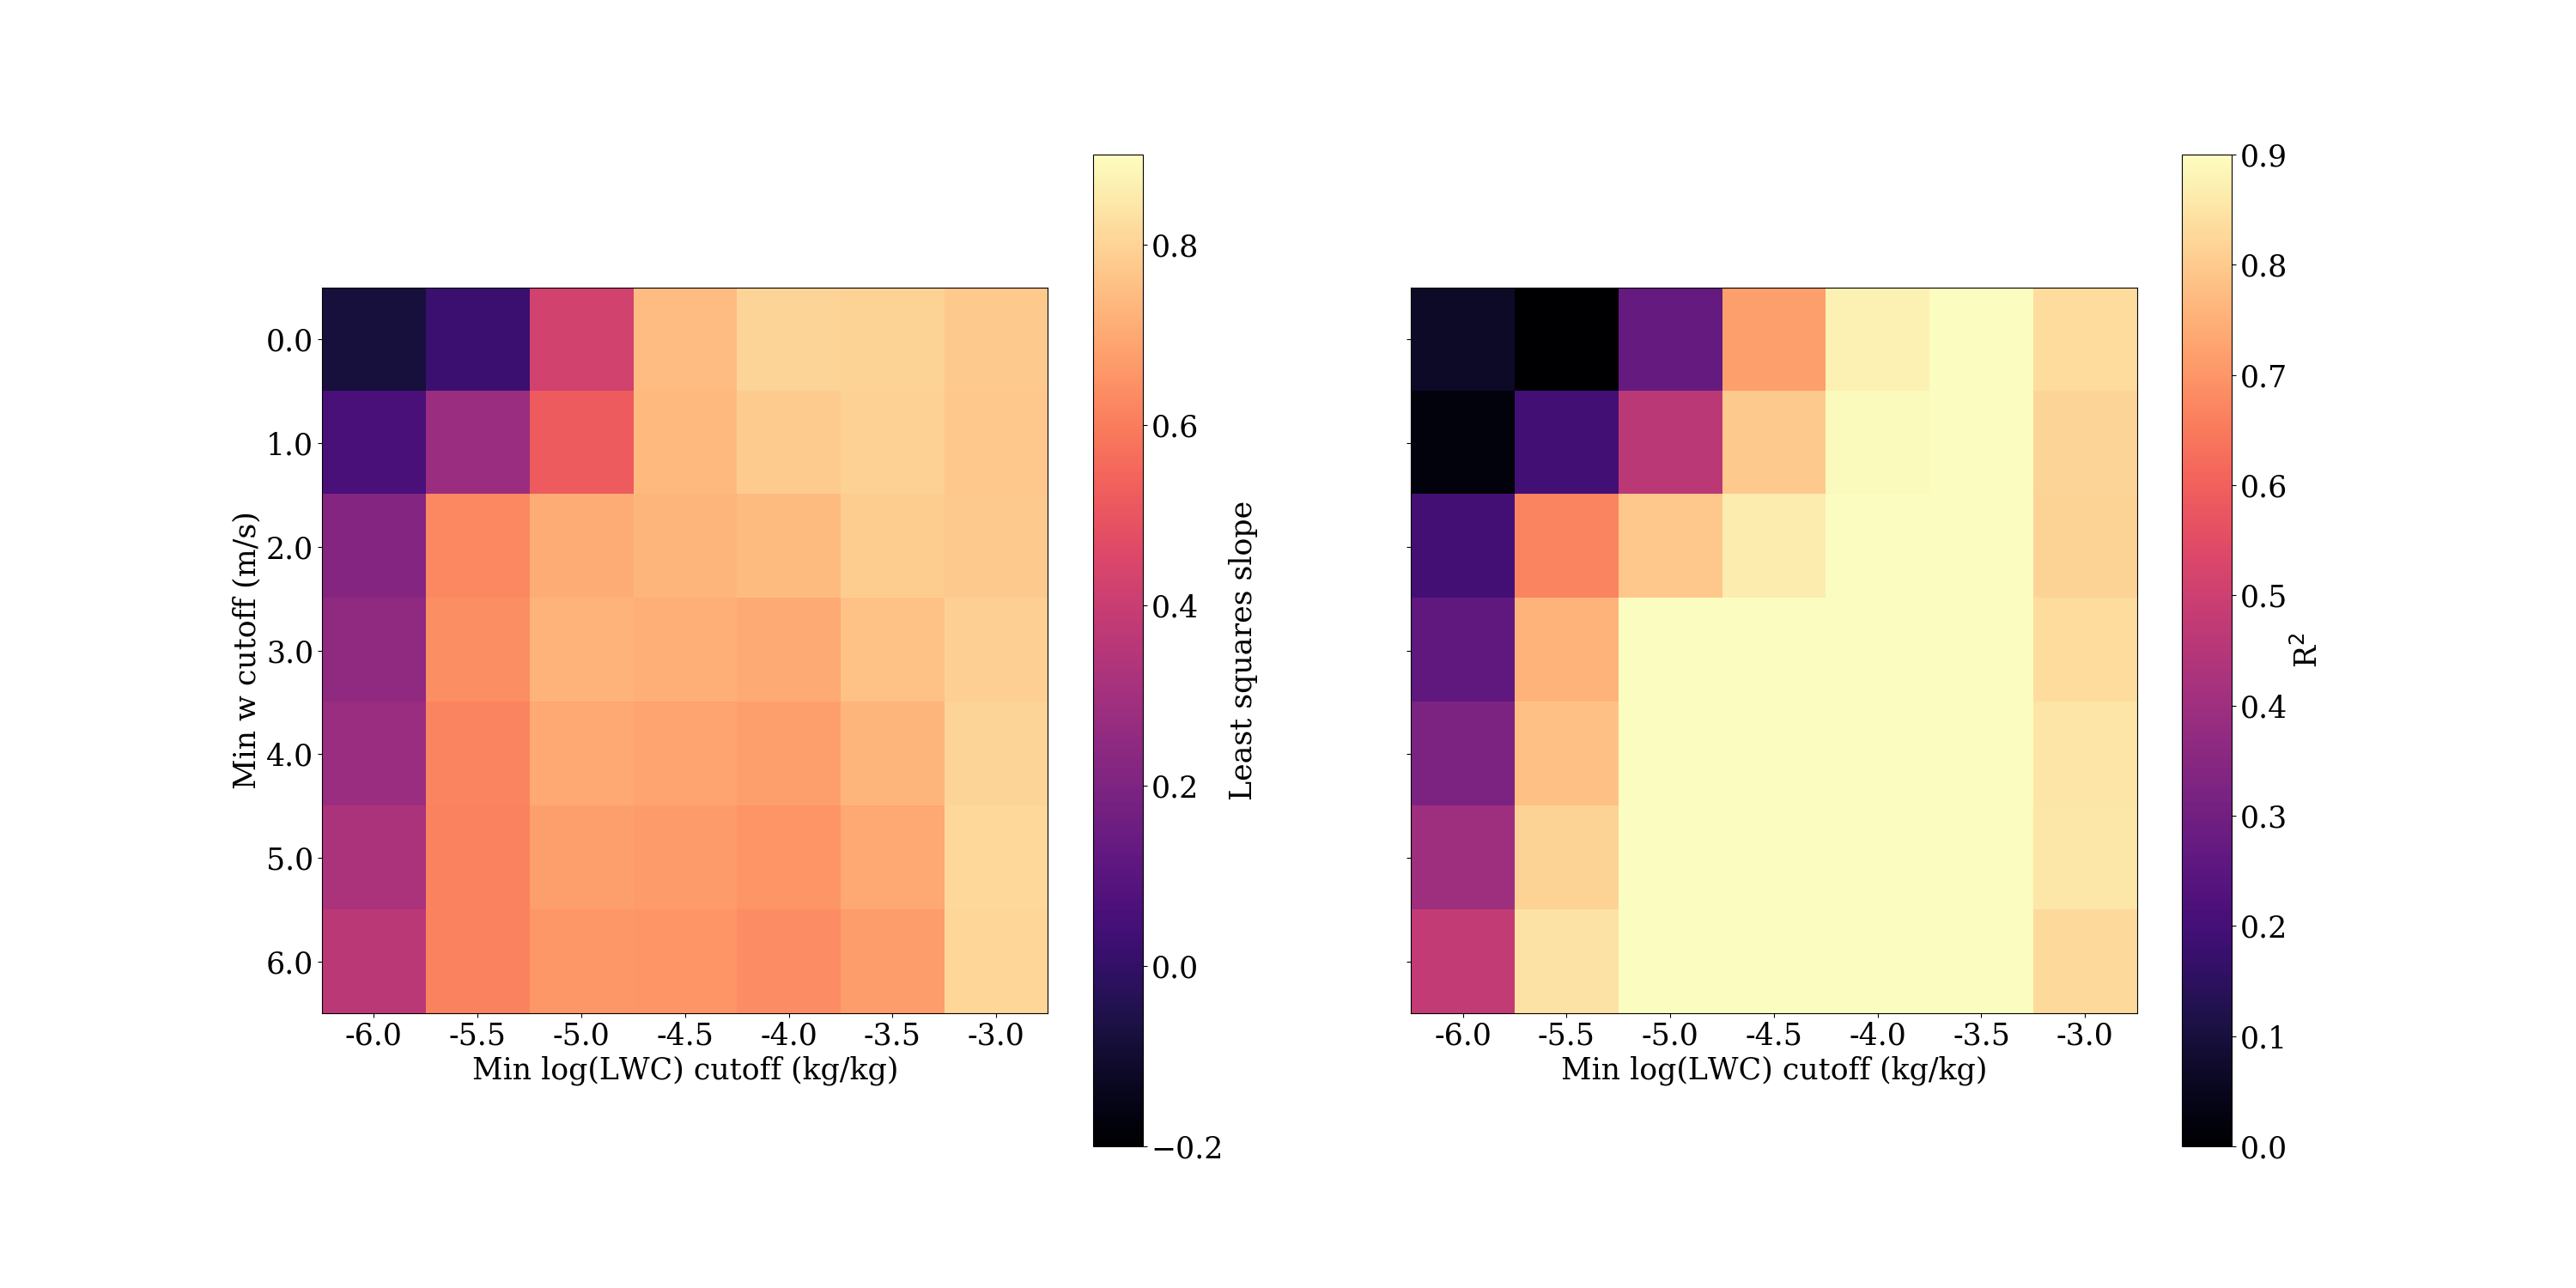
\includegraphics[width=\textwidth]{revmywrf/v1_FINAL_from_data_regres_param_heatmaps_Unpolluted_figure.png}
		\caption{Unpolluted case.}
		\label{regresheatmapunpoll}
	\end{subfigure}
	\begin{subfigure}{1\textwidth}
		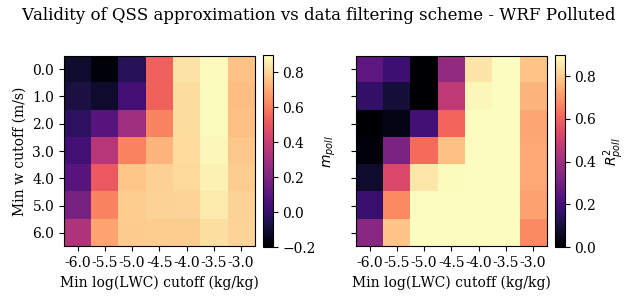
\includegraphics[width=\textwidth]{revmywrf/v1_FINAL_from_data_regres_param_heatmaps_Polluted_figure.png}
		\caption{Polluted case.}
		\label{regresheatmappoll}
	\end{subfigure}
	\caption{Heatmaps used to evaluate regime in which the QSS approximation gives a good estimate for the true SS. The parameters used to judge the quality of this estimate are the least-squares linear regression slope $m$ and correlation coefficient $R^2$ when plotting the true SS output from the simulation data ($SS_{WRF}$) versus the value derived from the WSS formula ($SS_{QSS}$) - see methods section. Values on the horizontal and vertical axes represent, respectively, minimum $LWC$ and $w$ cutoffs used to filter WRF simulation data. In all cases we additionally restrict our consideration to points with temperature above 273 K. Results are shown for model runs labeled in Fan et al as a) `C\_PI' (Unpolluted; subscript `unpoll') and b) `C\_BG' (Polluted; subscript `poll').}
	\label{regresheatmap}
\end{figure}

\begin{figure}[ht]
    \centering
    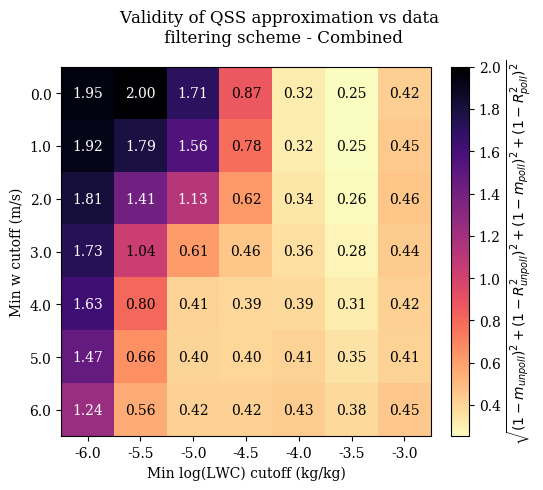
\includegraphics[width=9cm]{revmywrf/v1_FINAL_from_data_dist_heatmap_figure.png}
    \caption{A synthesis of the information in all four panels of Figure \ref{regresheatmap}. Here, the heatmap color corresponds to the Euclidean distance in the 4-dimensional space of tuples $(m_{unpoll}, R^2_{unpoll}, m_{poll}, R^2_{poll})$ from the ideal point $(1, 1, 1, 1)$. Numerical values of this distance are also given as annotations to aid in distinguishing similar colors. Horizontal and vertical axes are as described in Figure \ref{regresheatmap}.}
    \label{distheatmap}
\end{figure}

\begin{figure}[ht]
	\centering
	\begin{subfigure}{0.7\textwidth}
		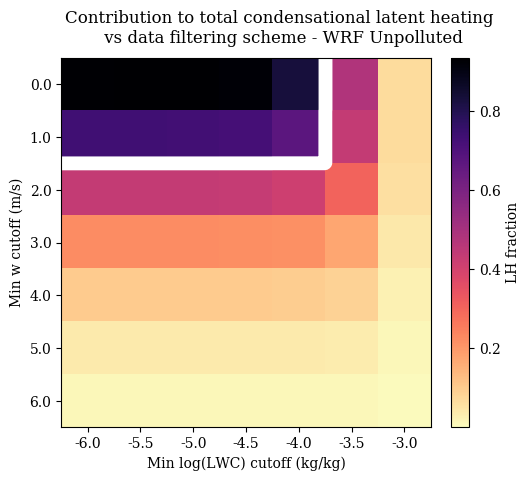
\includegraphics[width=\textwidth]{revmywrf/v1_FINAL_from_data_lh_frac_heatmap_Unpolluted_figure.png}
		\caption{Unpolluted case.}
		\label{lhheatmapunpoll}
	\end{subfigure}
	\begin{subfigure}{0.7\textwidth}
		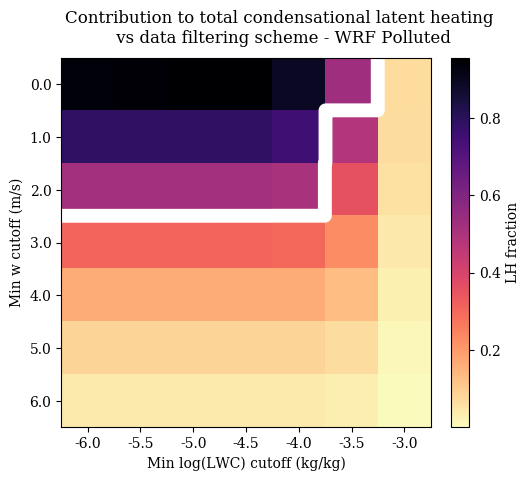
\includegraphics[width=\textwidth]{revmywrf/v1_FINAL_from_data_lh_frac_heatmap_Polluted_figure.png}
		\caption{Polluted case}
		\label{lhheatmappoll}
	\end{subfigure}
	\caption{Heatmaps to evaluate the fraction of domain-wide positive (i.e. condensational) latent heating attributed to points selected through the data filter. The higher the fraction, the more confidence we have (in an unquantified sense) that we are capturing a complete picture of the convection which sets the temperature profile in the troposphere. The horizontal and vertical axes are as described in Figure \ref{regresheatmap}. The white contour line indicates the region of the heatmap where the LH fraction is $> 50\%$.}
	\label{lhheatmap}
\end{figure}

\begin{figure}[ht]
	\centering
	\begin{subfigure}{0.7\textwidth}
		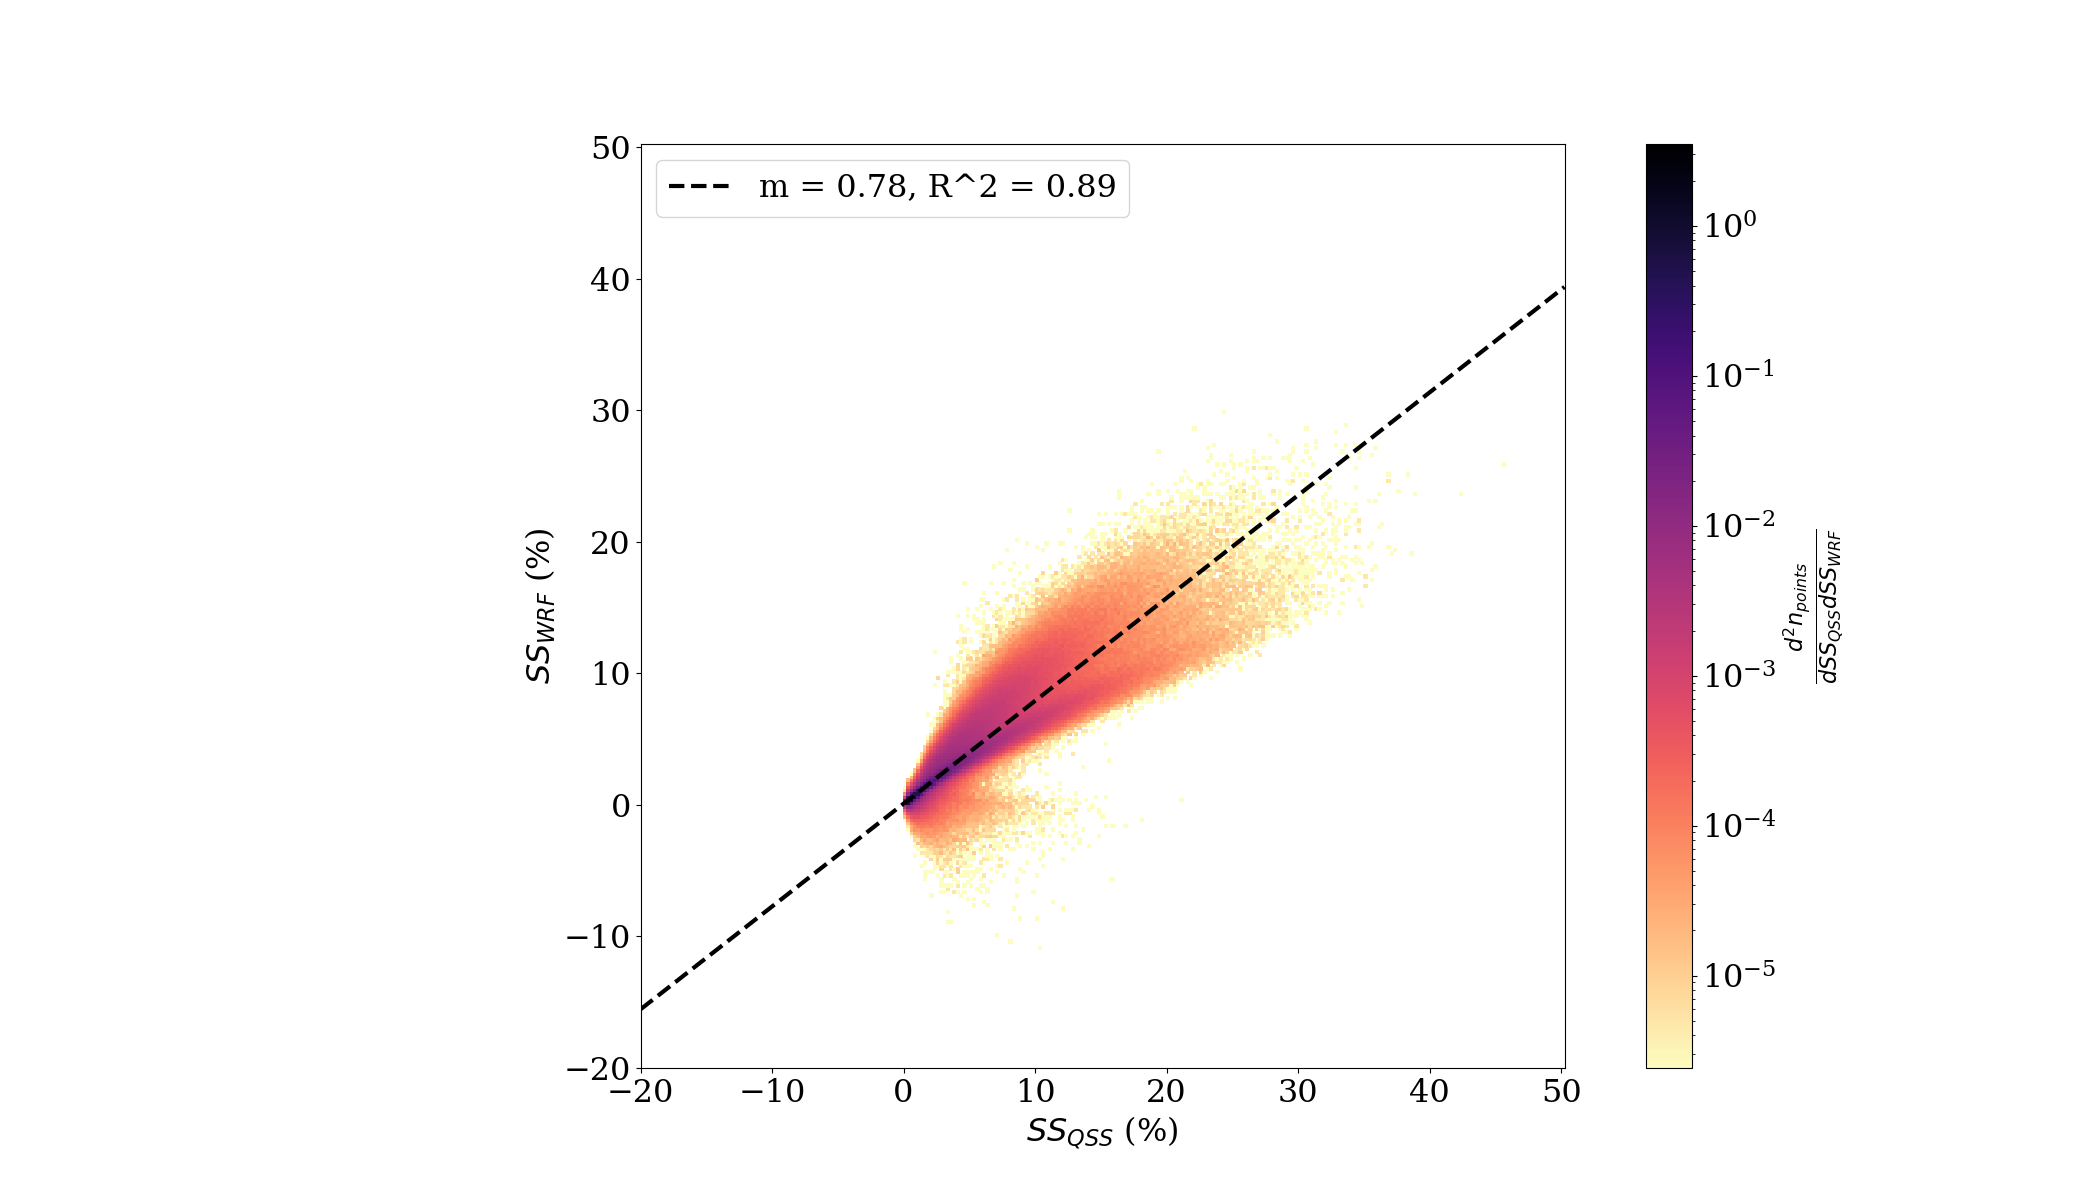
\includegraphics[width=\textwidth]{revmywrf/v10_FINAL_heatmap_ss_qss_vs_ss_wrf_Unpolluted_figure.png}
		\caption{Unpolluted case.}
		\label{wrfvsqssunpoll}
	\end{subfigure}
	\begin{subfigure}{0.7\textwidth}
		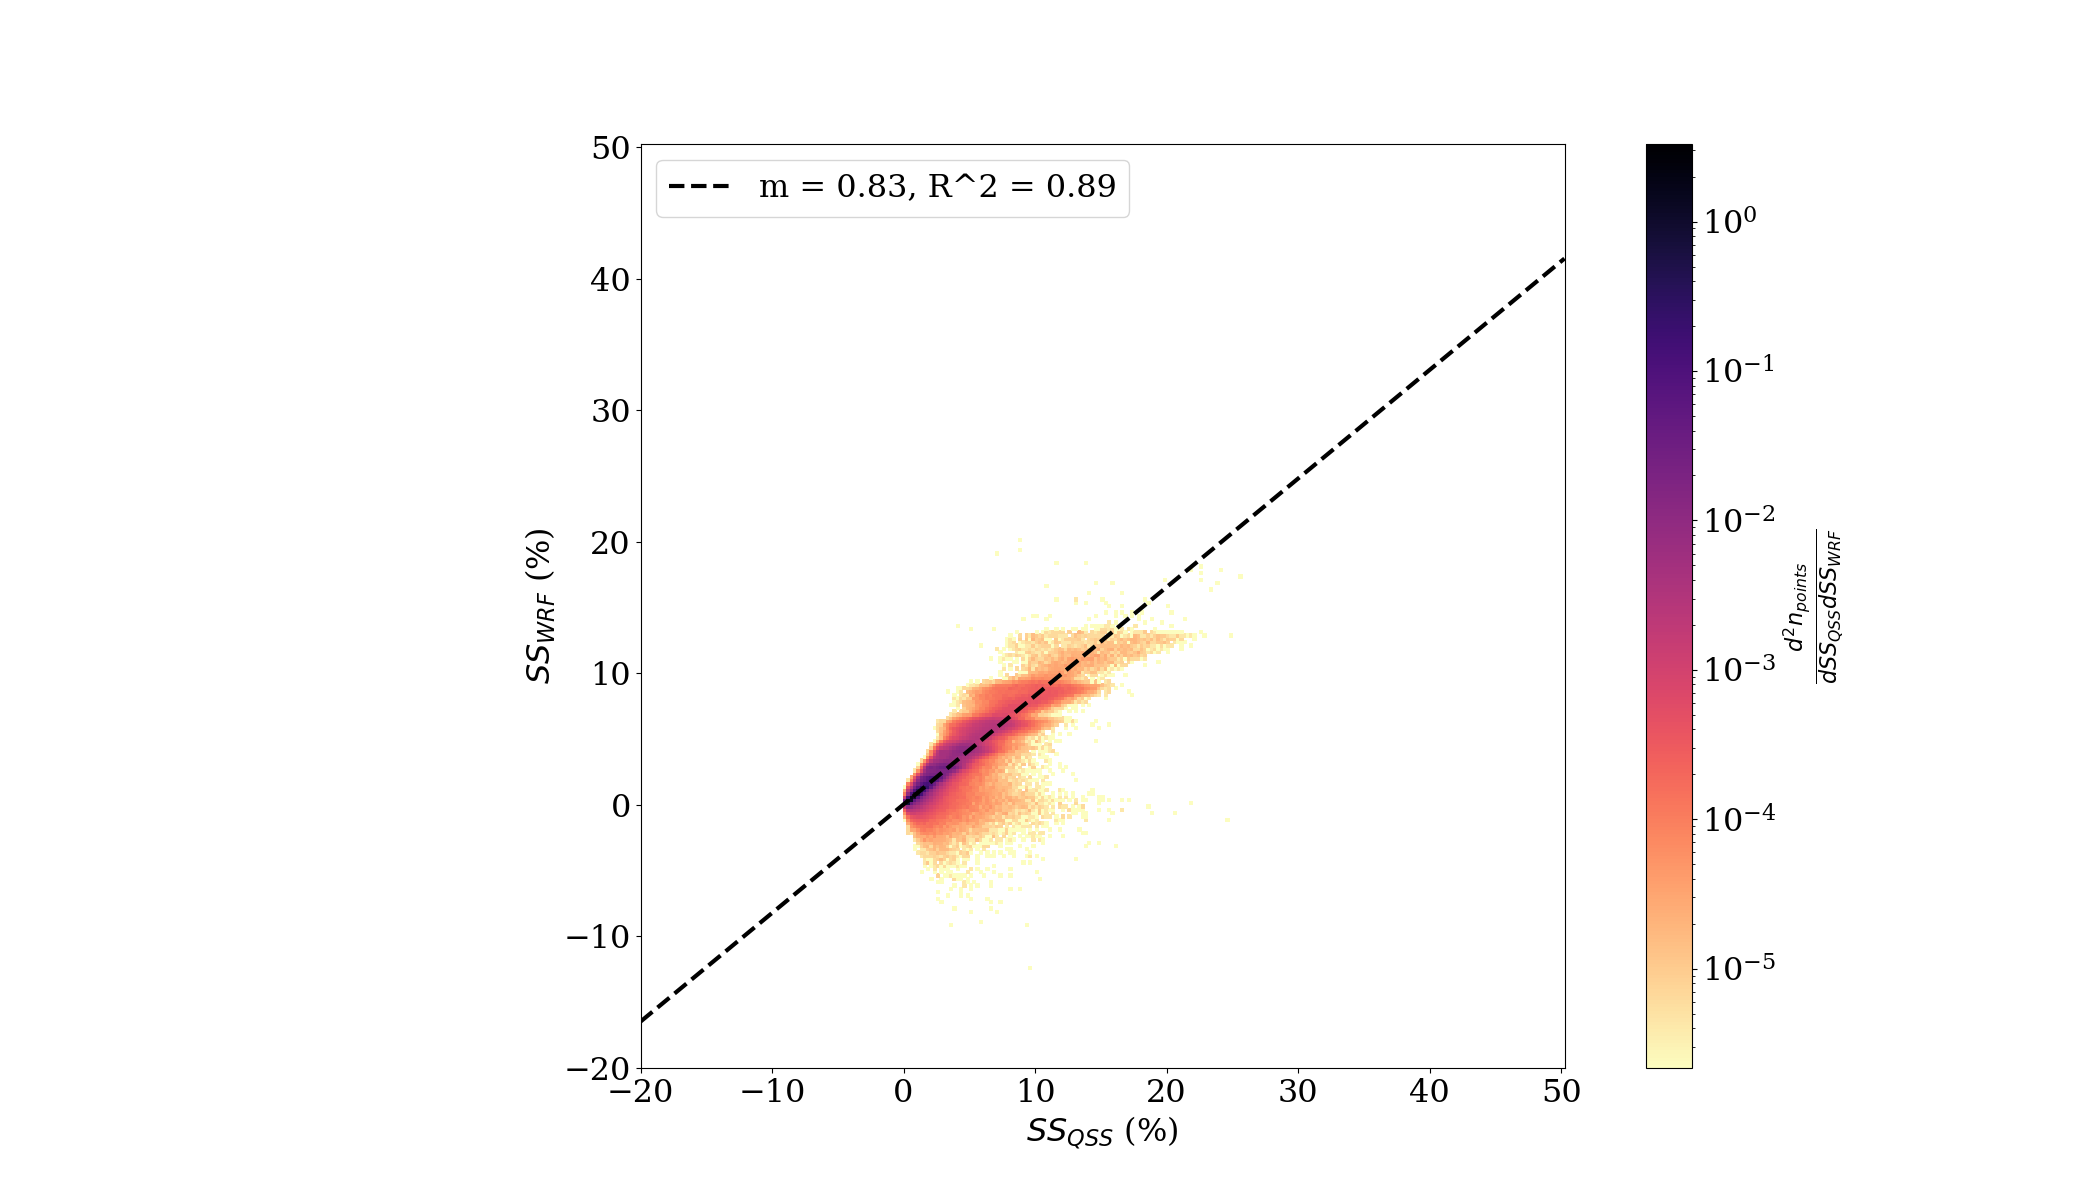
\includegraphics[width=\textwidth]{revmywrf/v10_FINAL_heatmap_ss_qss_vs_ss_wrf_Polluted_figure.png}
		\caption{Polluted case.}
		\label{wrfvsqsspoll}
	\end{subfigure}
	\caption{Plot of $SS_{QSS}$ versus $SS_{WRF}$ using the filtering scheme described in the main text. Dashed line shows the fit from least-squares linear regression. Color denotes the density of data points; note the scale is logarithmic in this figure. The majority of points are clustered near the origin.}
	\label{wrfvsqss}
\end{figure}

\begin{figure}[ht]
	\centering
	\begin{subfigure}{0.7\textwidth}
		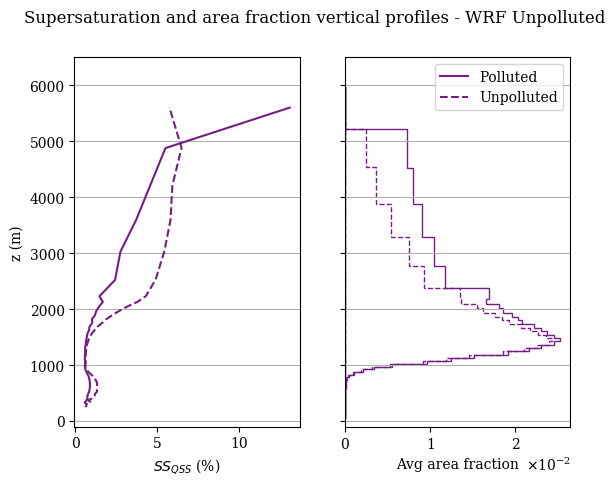
\includegraphics[width=\textwidth]{revmywrf/v20_FINAL_bipanel_ss_qss_vs_z_allpts_figure.png}
		\caption{}
		\label{wrfbipanelallpts}
	\end{subfigure}
	\begin{subfigure}{0.7\textwidth}
		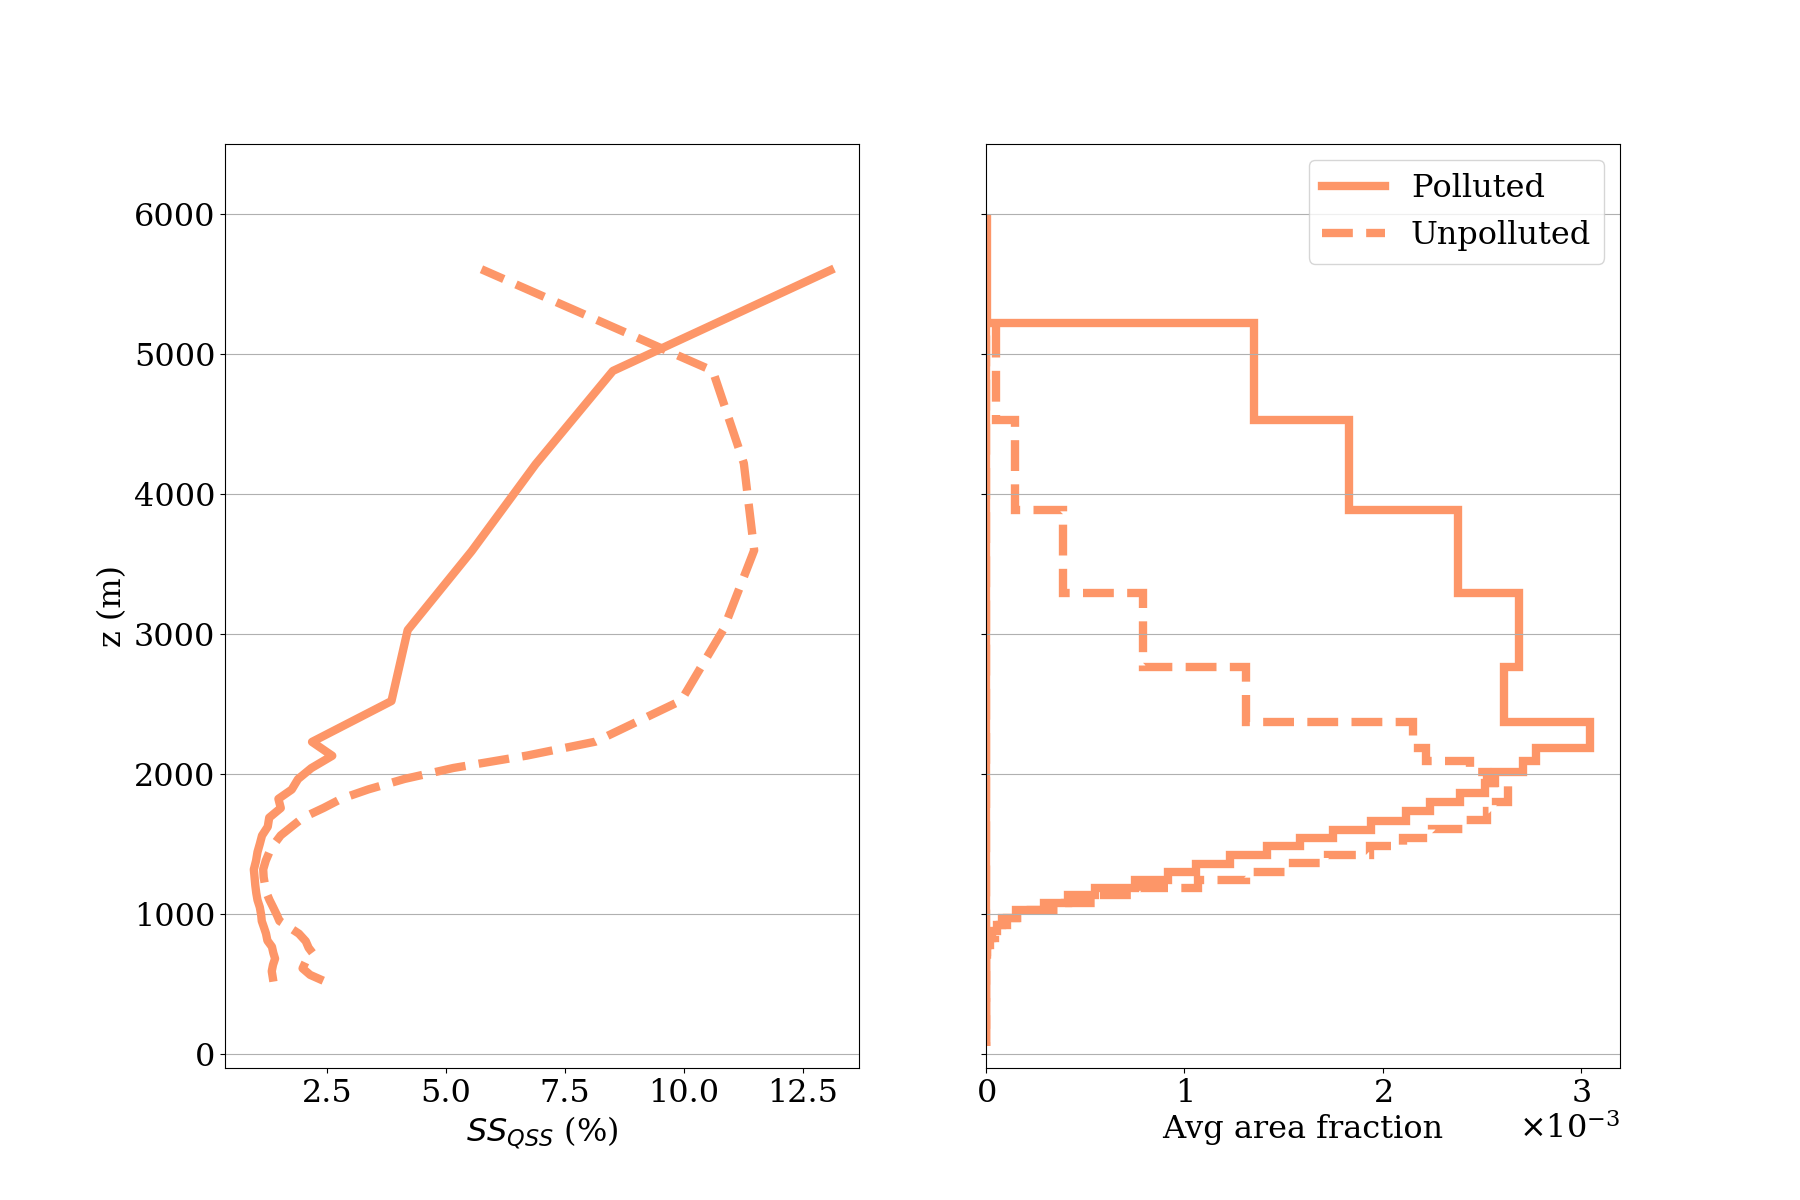
\includegraphics[width=\textwidth]{revmywrf/v20_FINAL_bipanel_ss_qss_vs_z_up10perc_figure.png}
		\caption{}
		\label{wrfbipanelup50perc}
	\end{subfigure}
	\caption{This figure serves to verity that our data filtering scheme yields SS profiles similar to those obtained by Fan et al (c.f. Figure 4 of that paper). Using a) all filtered data points and b) only the top 10 percentiles of filtered data points as measured by $w$ (see text for details), the latter being aligned with the analysis method of Fan et al. Left hand panels show $SS_{QSS}$ averaged across time and horizontal spatial coordinates. Right hand panels show time-averaged area fraction occupied by filtered data points. Note that $z$ interval width scales logarithmically with $z$, in accordance with the WRF grid spacing. We observe that our filtering scheme indeed recovers average $SS_{QSS}$ values on the order of 10\% as reported in Fan's paper. The dropoff in area fraction in (a) at higher altitudes is due to a fairly sharp peak in $LWC$ around 2-3 km (see Figure \ref{lwcprof} in Supplementary section).}
	\label{wrfbipanel}
\end{figure}

\begin{figure}[ht]
    \centering
    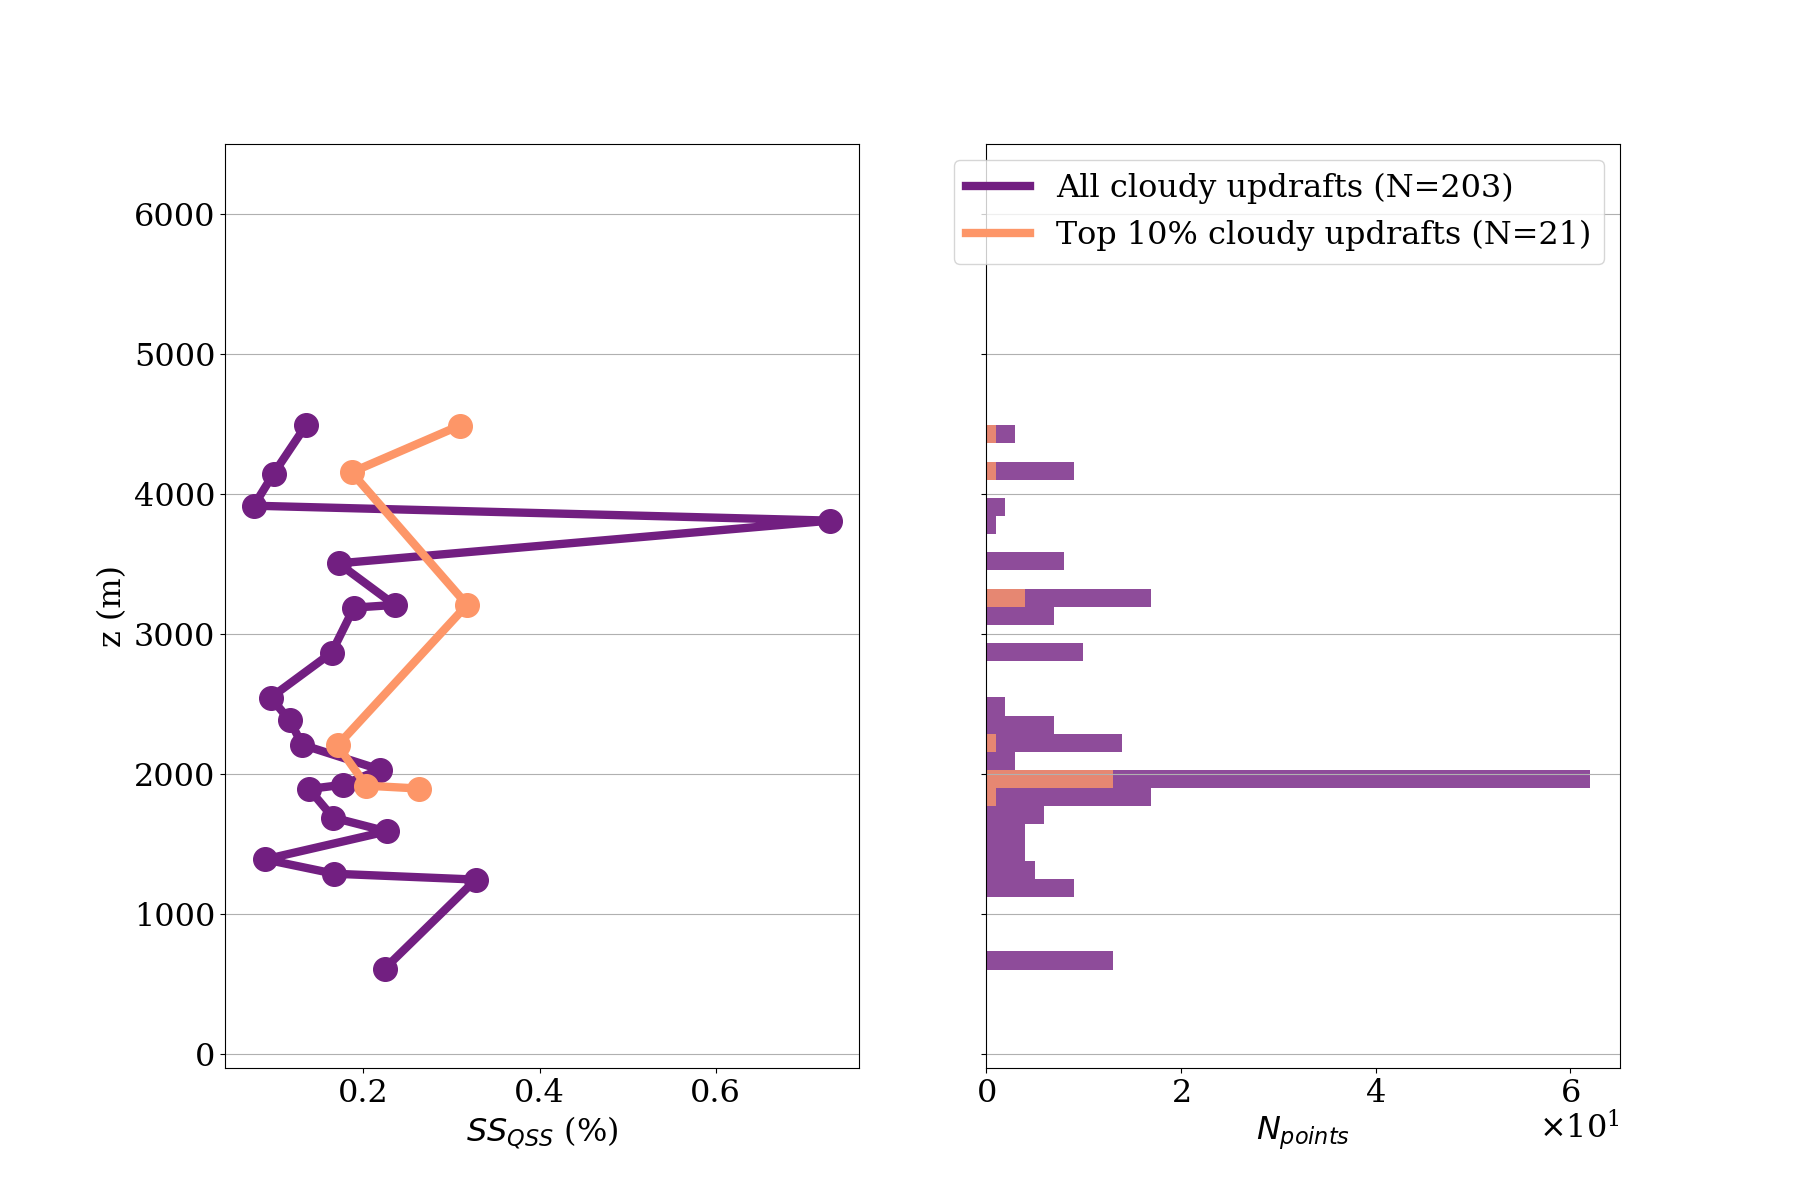
\includegraphics[width=9cm]{revhalo/v8_FINAL_combined_bipanel_ss_qss_vs_z_figure.png}
    \caption{This figure serves to determine whether the high-SS values found in the WRF simulation output indeed occur in nature. Left hand panel shows $SS_{QSS}$ averaged across all filtered data points from HALO flight campaign (all dates combined), as well as across only the top 10 percentiles of those filtered data points as measured by $w$ (see text for details). Right hand panel shows the number of points in each $z$ interval (constant with respect to $z$) used in the analysis. We do not find any points in the $SS_{QSS}$ profile with values above 1\%, even when restricting to only the top 10 percentiles of updrafts.}
    \label{halobipanel}
\end{figure}

\begin{figure}[ht]
    \centering
    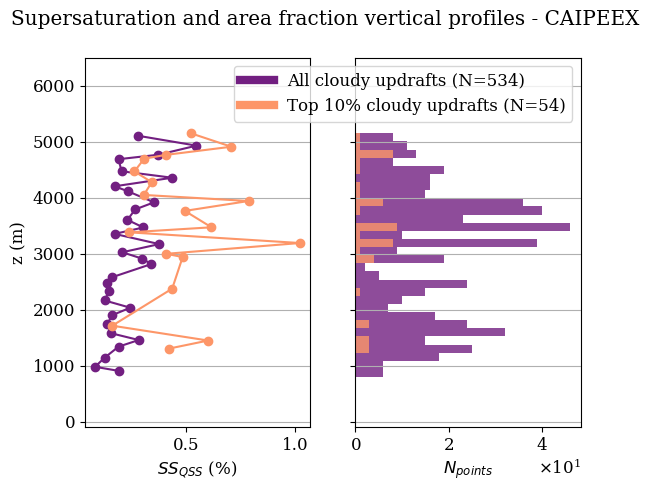
\includegraphics[width=9cm]{revcaipeex/v8_FINAL_combined_bipanel_ss_qss_vs_z_figure.png}
    \caption{Analagous to Figure \ref{halobipanel} but using experimental data from the CAIPEEX flight campaign. The only difference in the analysis for this dataset (relative to for the HALO dataset) is that we did not have access to size-resolved rain drop spectra (see text for detailed discussion). We do not find any points in the $SS_{QSS}$ profile with values above 1\% for the entire filtered data set, with only one point in the profile exceeding 1\% for the top 10 percentiles of updrafts.}
    \label{caipeexbipanel}
\end{figure}

\begin{figure}[ht]
    \centering
    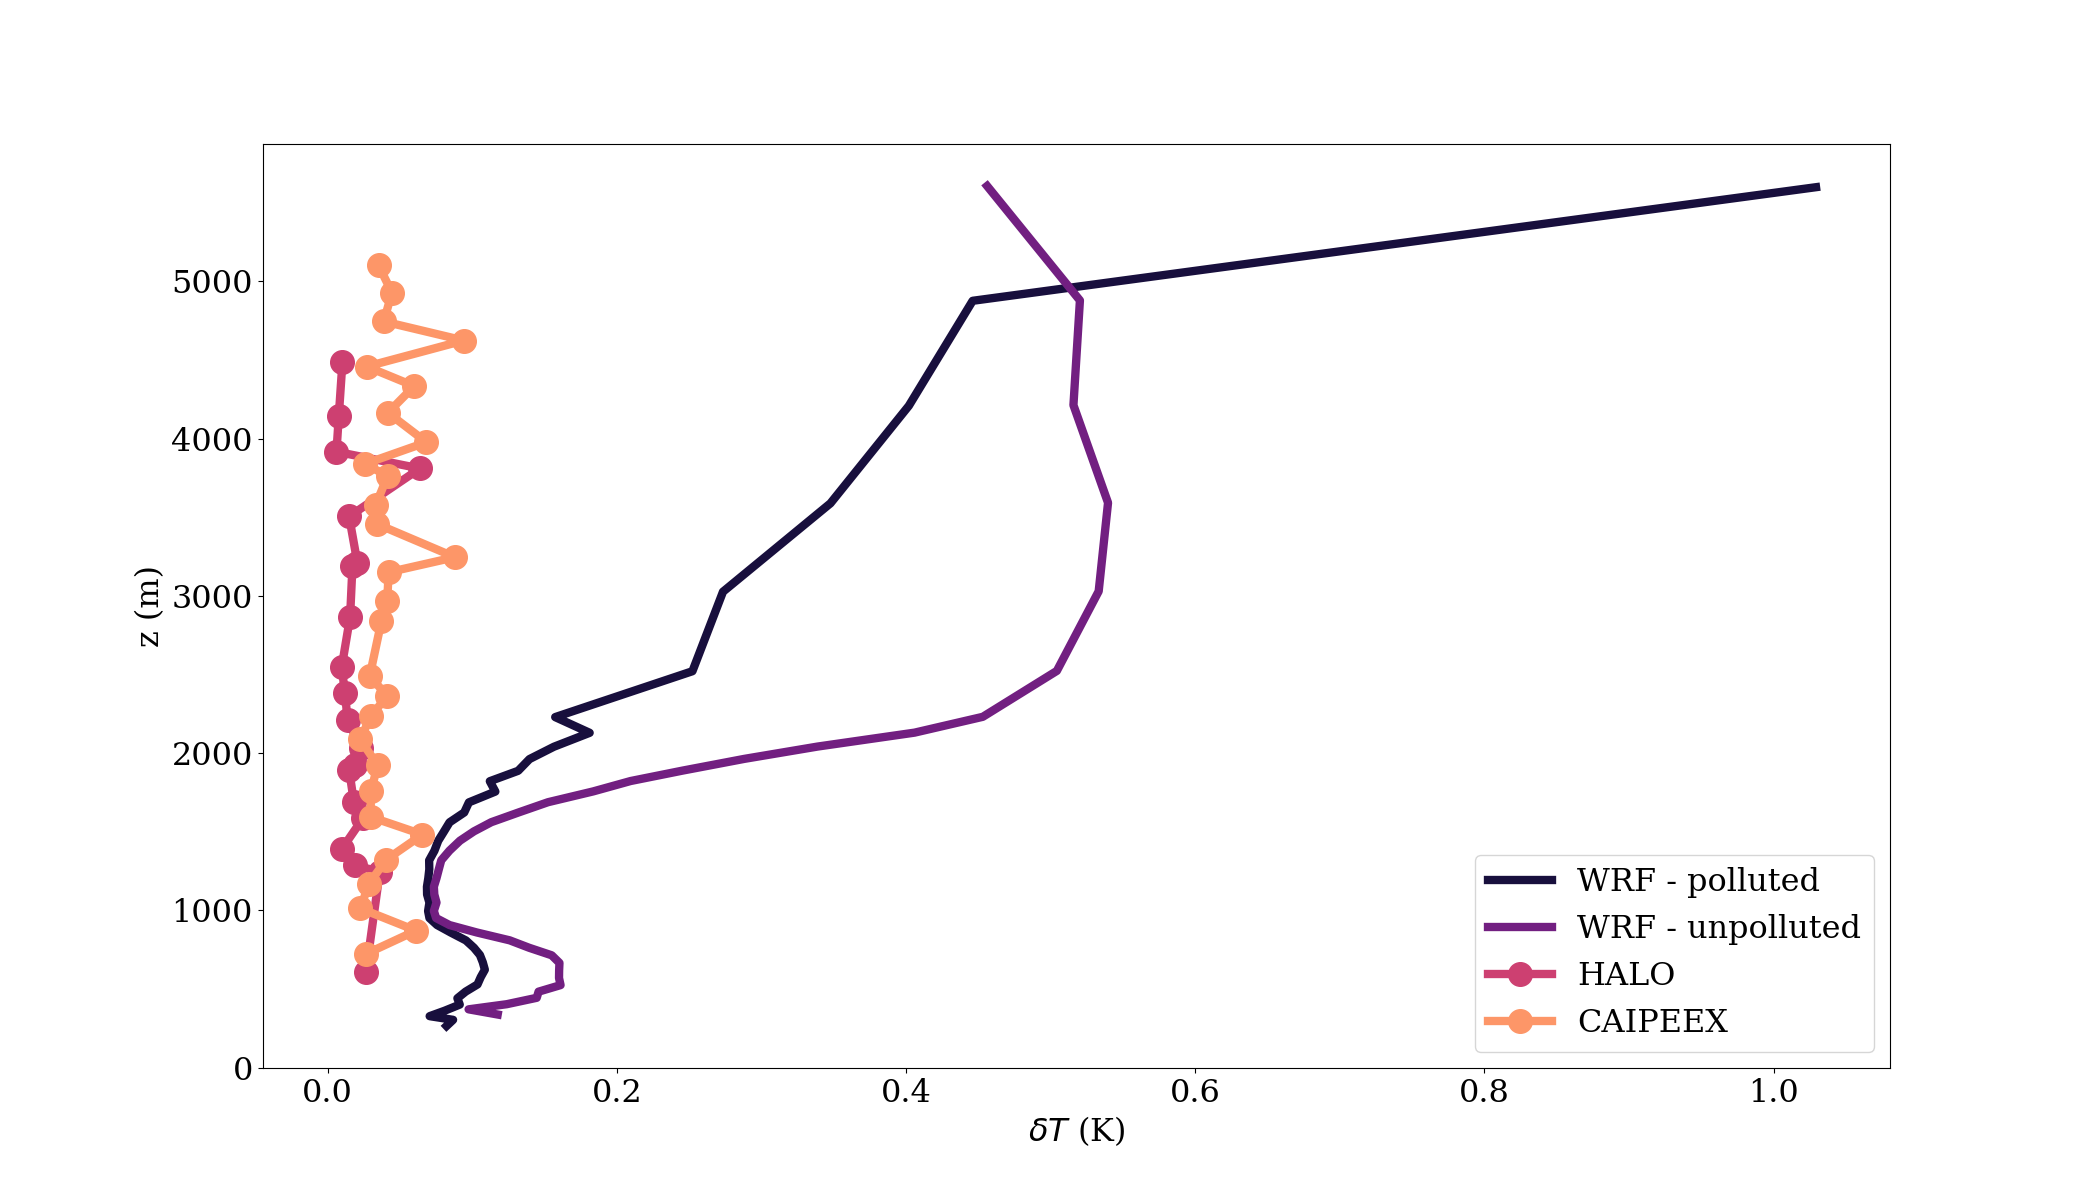
\includegraphics[width=12cm]{revmywrf/v2_FINAL_combined_dT_profile_figure.png}
    \caption{Profiles for $\delta T$ of a non-supersaturated ($RH=1$) parcel ascending in an environment with SS profiles shown in Figures \ref{wrfbipanel}-\ref{caipeexbipanel}, using Equation \ref{dCAPE}. SS profiles for HALO and CAIPEEX are plotted with markers so as not to obscure intervals with missing data. We find that the buoyancy of this hypothetical parcel in nature is far lower than in the simulations, casting doubt on the real validity of the WPIM as described in Fan et al.}
    \label{dTprofiles}
\end{figure}

\begin{figure}[ht]
	\centering
	\begin{subfigure}{0.7\textwidth}
		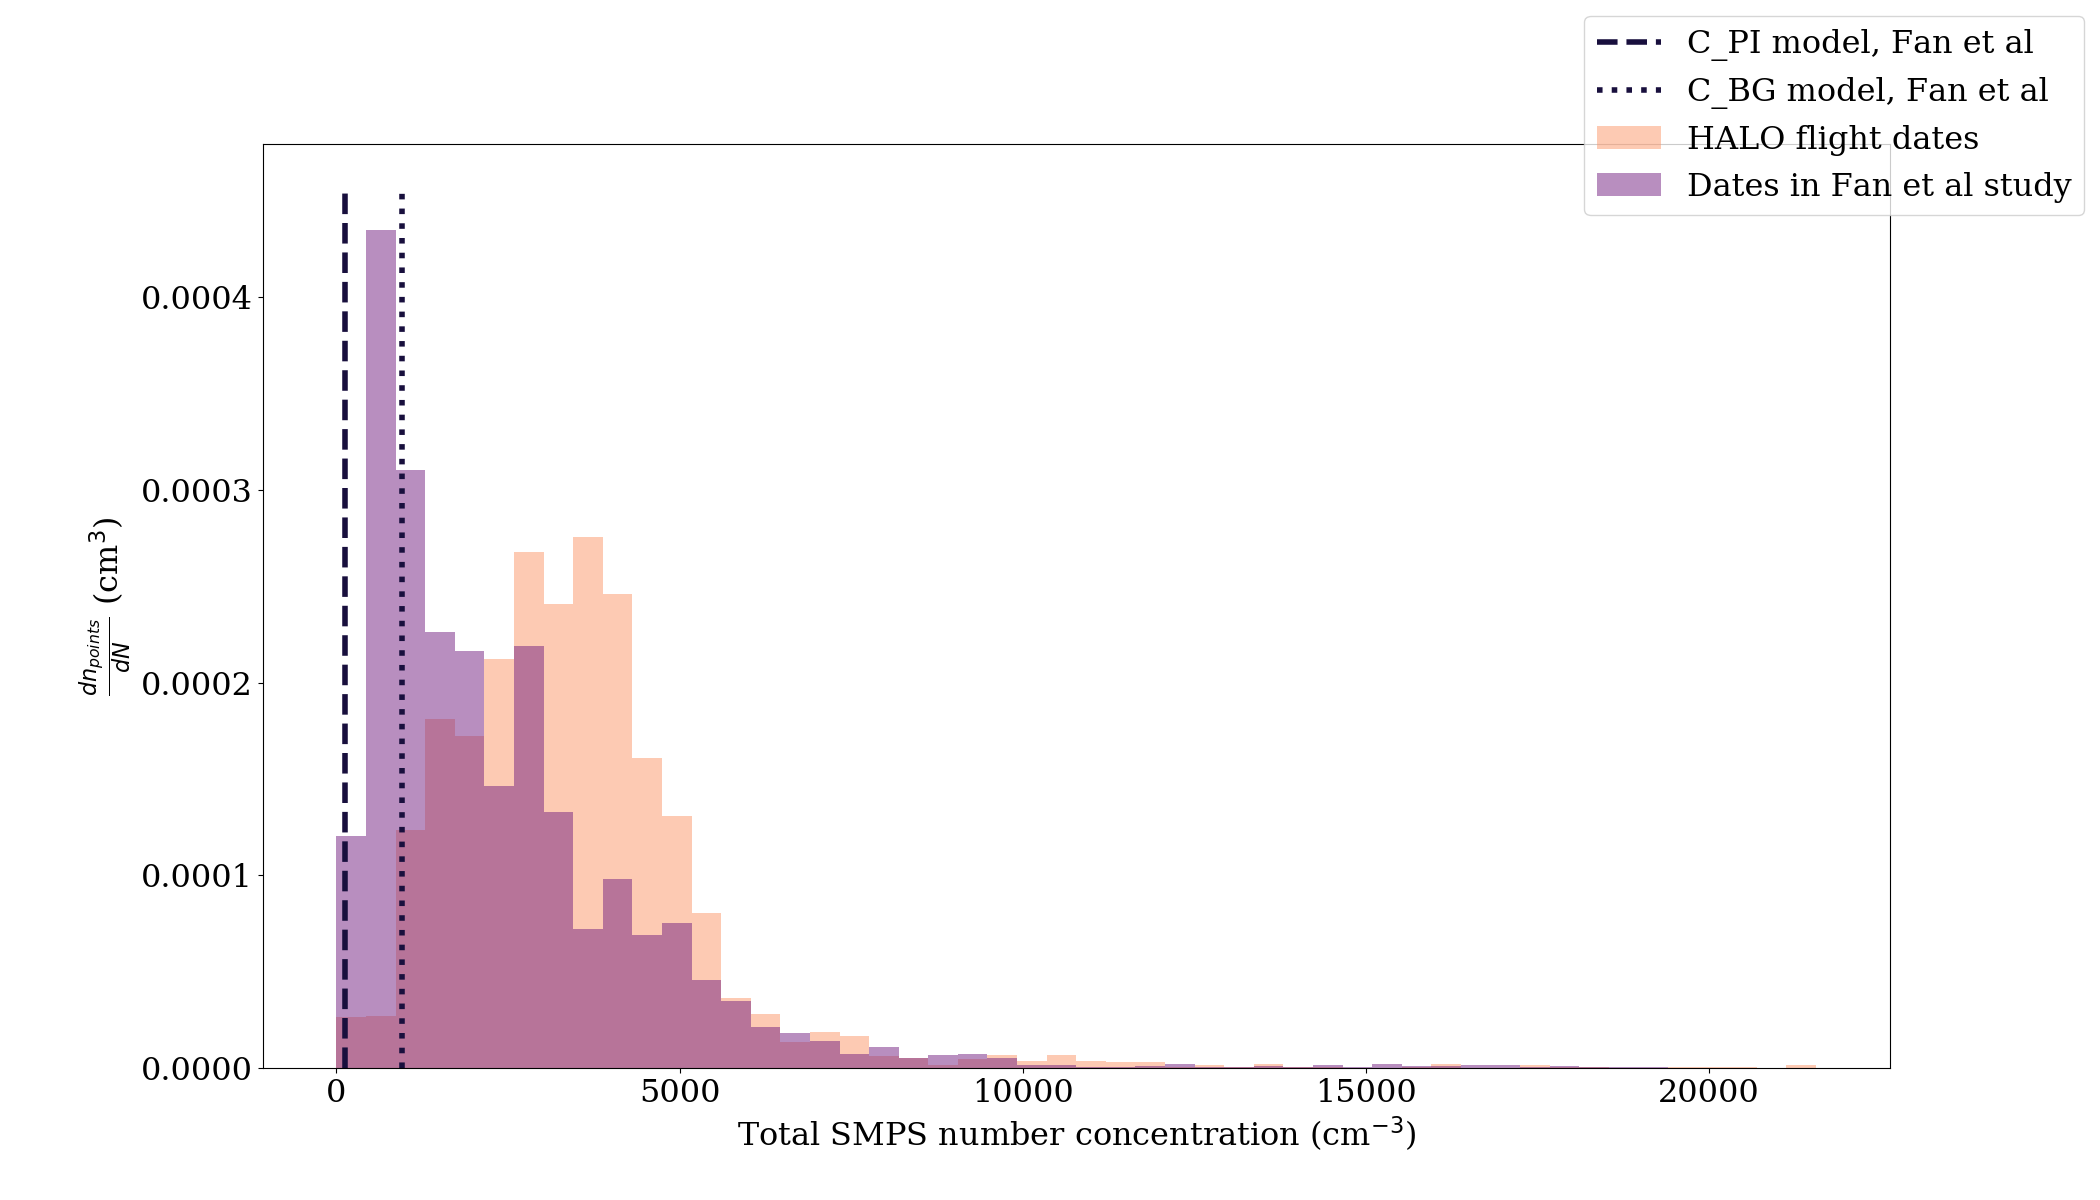
\includegraphics[width=\textwidth]{goama/v1_FINAL_tot_compare_nconc_hist_alldates_figure.png}
		\label{goamatothist}
		\caption{}
	\end{subfigure}
	\begin{subfigure}{0.7\textwidth}
		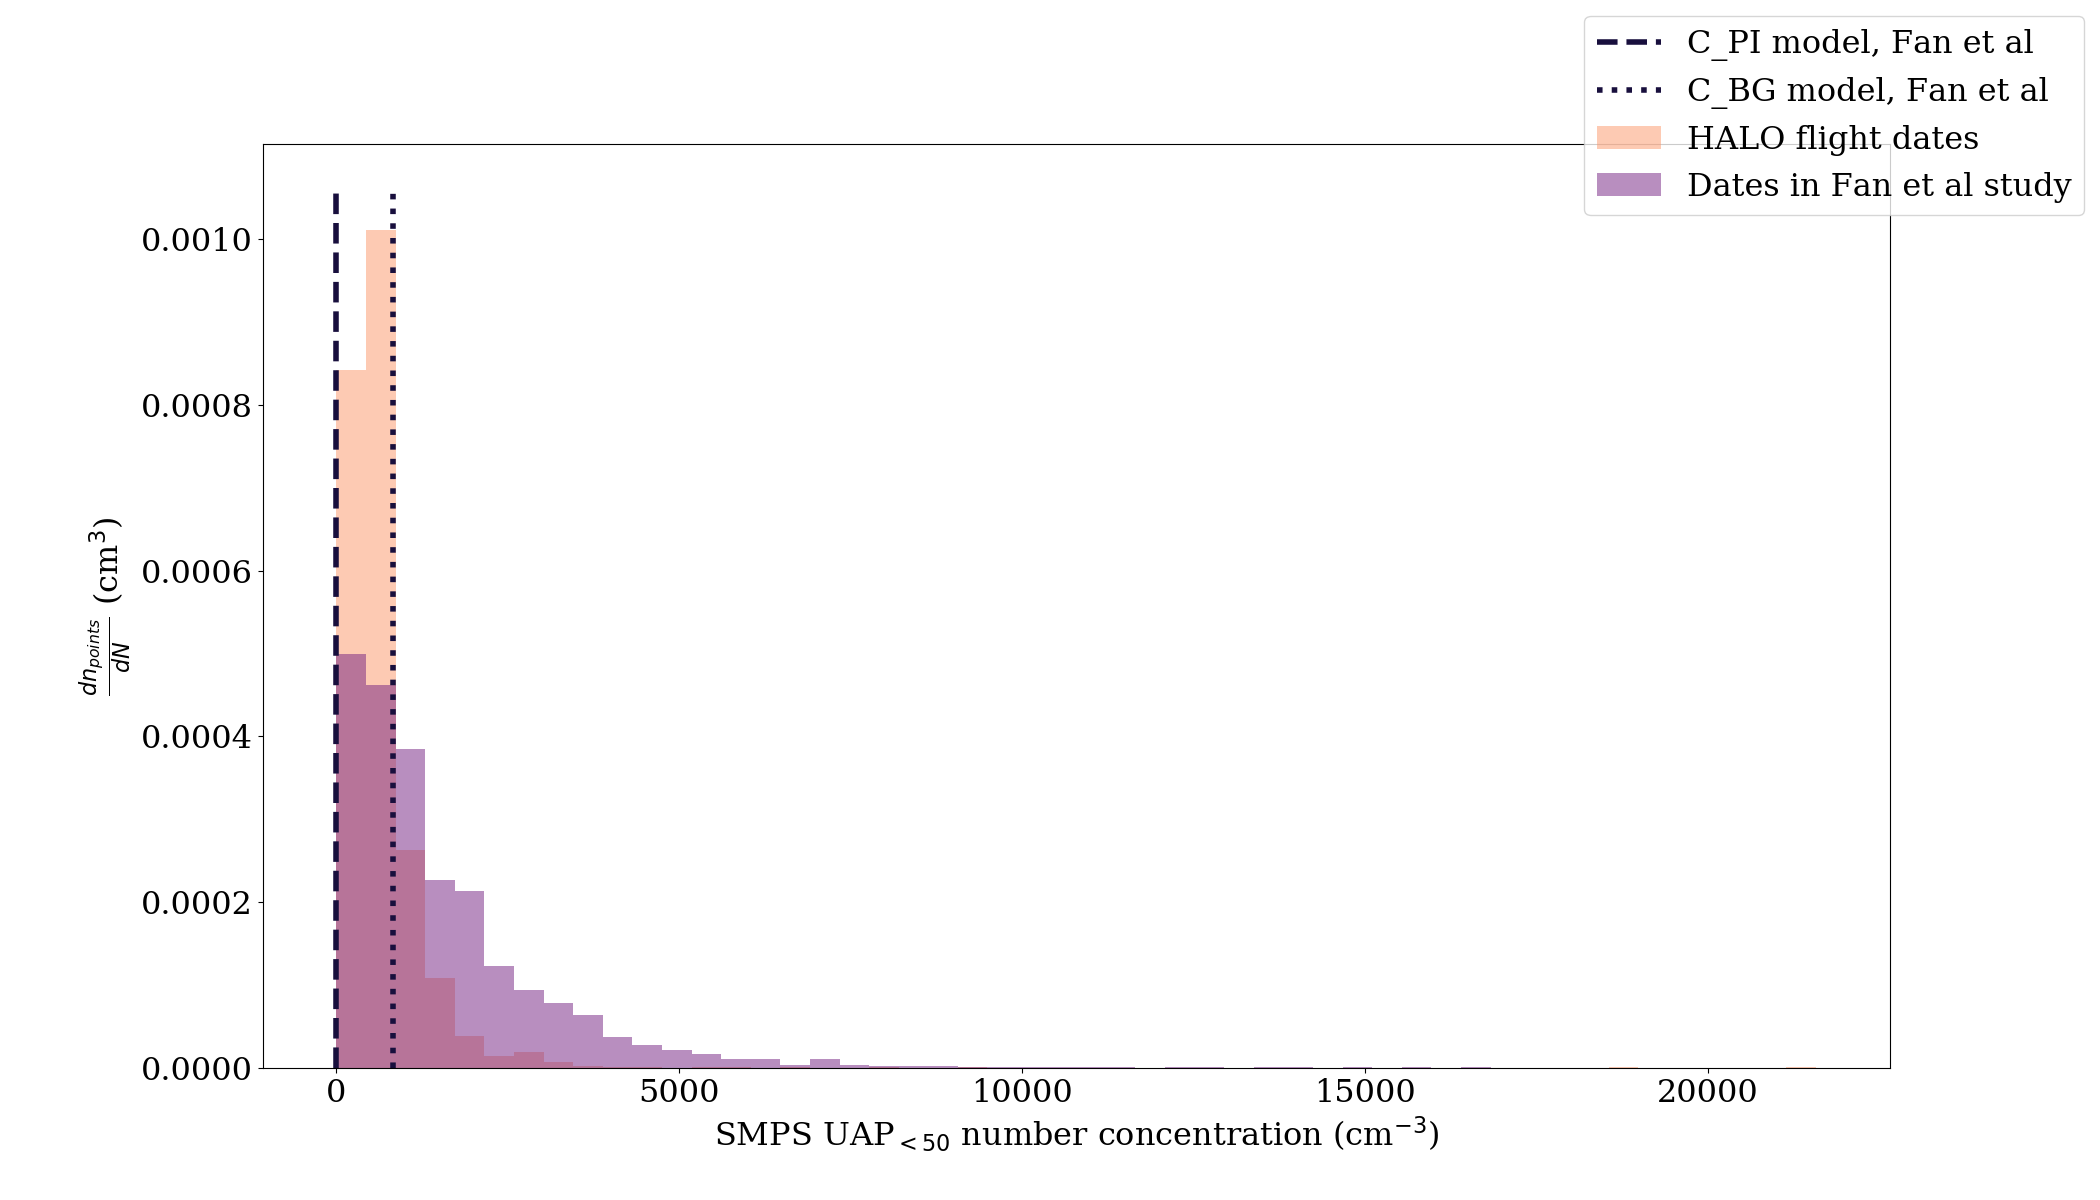
\includegraphics[width=\textwidth]{goama/v1_FINAL_uap50_compare_nconc_hist_alldates_figure.png}
		\label{goamauap50hist}
		\caption{}
	\end{subfigure}
	\caption{Distribution of aerosol concentration measurements by the ground-based SMPS at Manacapuru, Brazil; a) entire size range, b) only particles with diameter greater than 50nm. HALO flight dates are the same as those represented in Figure \ref{halobipanel} (see main text for details). Dashed (dotted) lines show initial concentrations in the BL of the WRF simulation of polluted (unpolluted) conditions. The unpolluted model aerosol concentrations are quite low relative to what is actually observed.}
	\label{goamahist}
\end{figure}

\begin{figure}[ht]
    \centering
    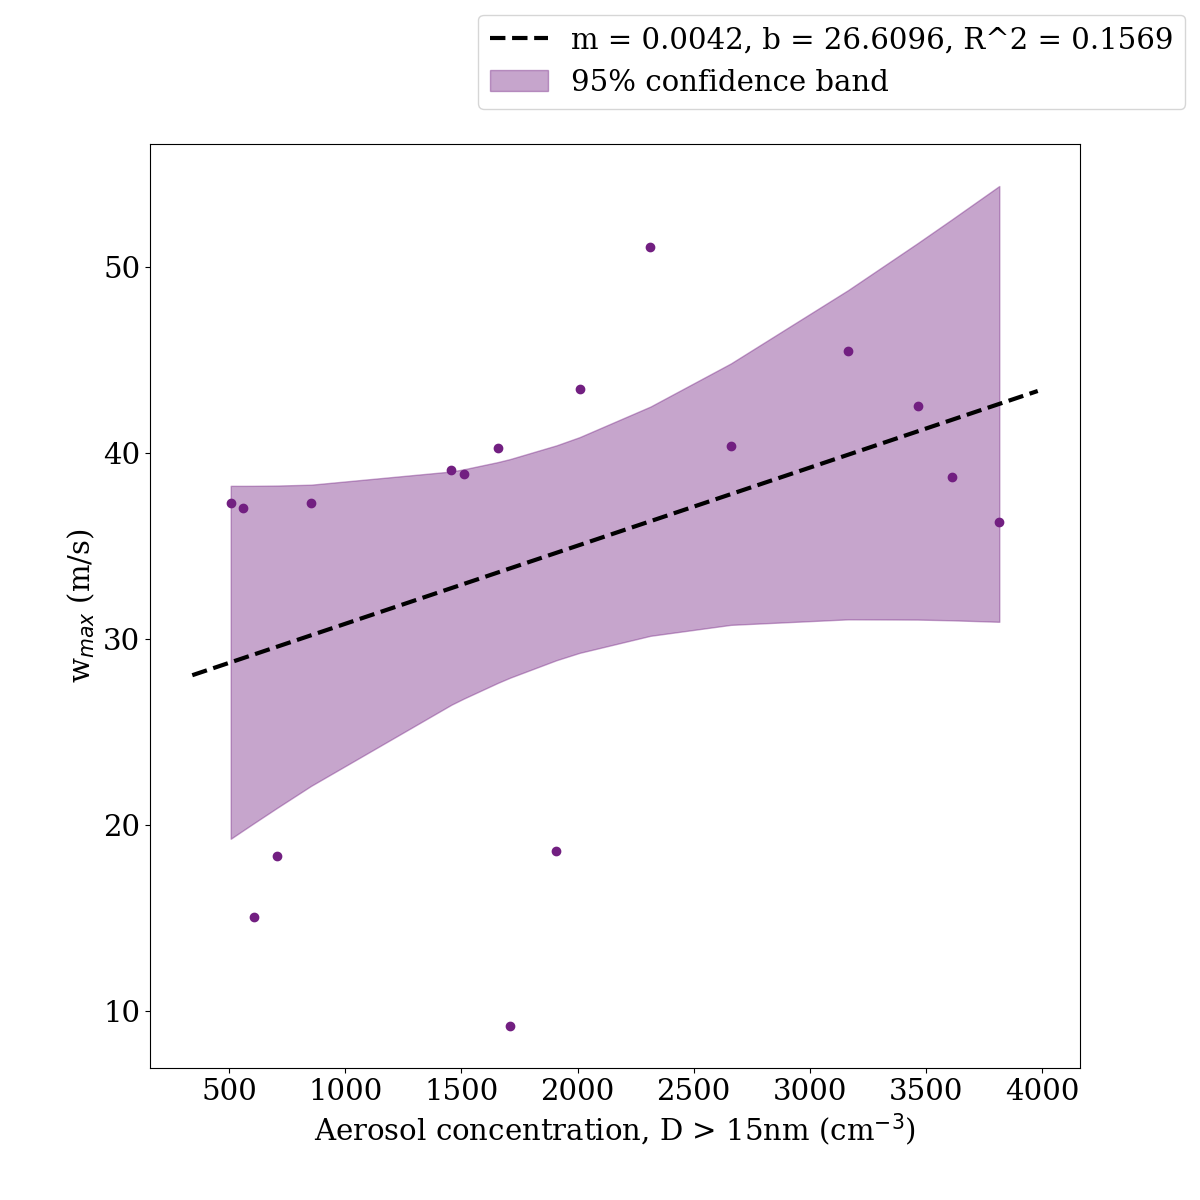
\includegraphics[width=12cm]{revhalo/v2_FINAL_fan_fig_s2a.png}
    \caption{Ground-based total (including UAP50) aerosol concentration measurements versus maximum vertical wind velocity in convective cores; reproduced from Figure S2(a) of \cite{Fan2018} with additional confidence bands our own. Note that a line with zero slope lies well within the confidence bands, corroborating the statistically insignificant p-value of the least-squares linear regression slope parameter.}
    \label{fans2a}
\end{figure}

\begin{figure}[ht]
    \centering
    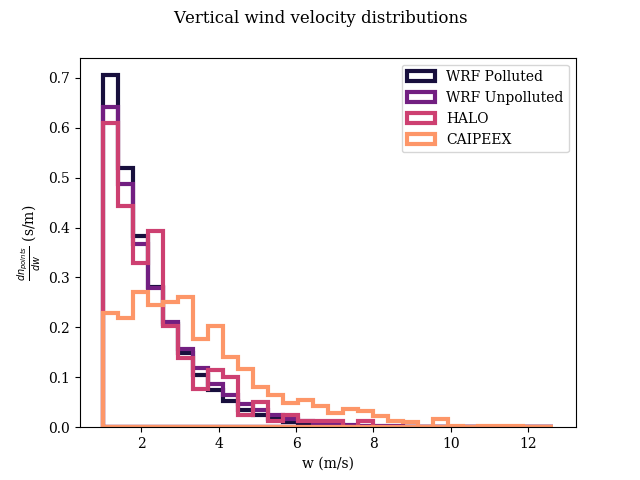
\includegraphics[width=12cm]{revmywrf/v3_FINAL_combined_w_hist_figure.png}
    \caption{Vertical wind velocity probability distributions from simulations and field campaigns, using filtering criteria outlined in the text. Experimental distributions are not qualtitatively different from those in the simulation.}
    \label{combinedwhist}
\end{figure}

\newpage
\clearpage

\section*{Supplementary}

\begin{figure}[ht]
	\centering
	\begin{subfigure}{0.7\textwidth}
		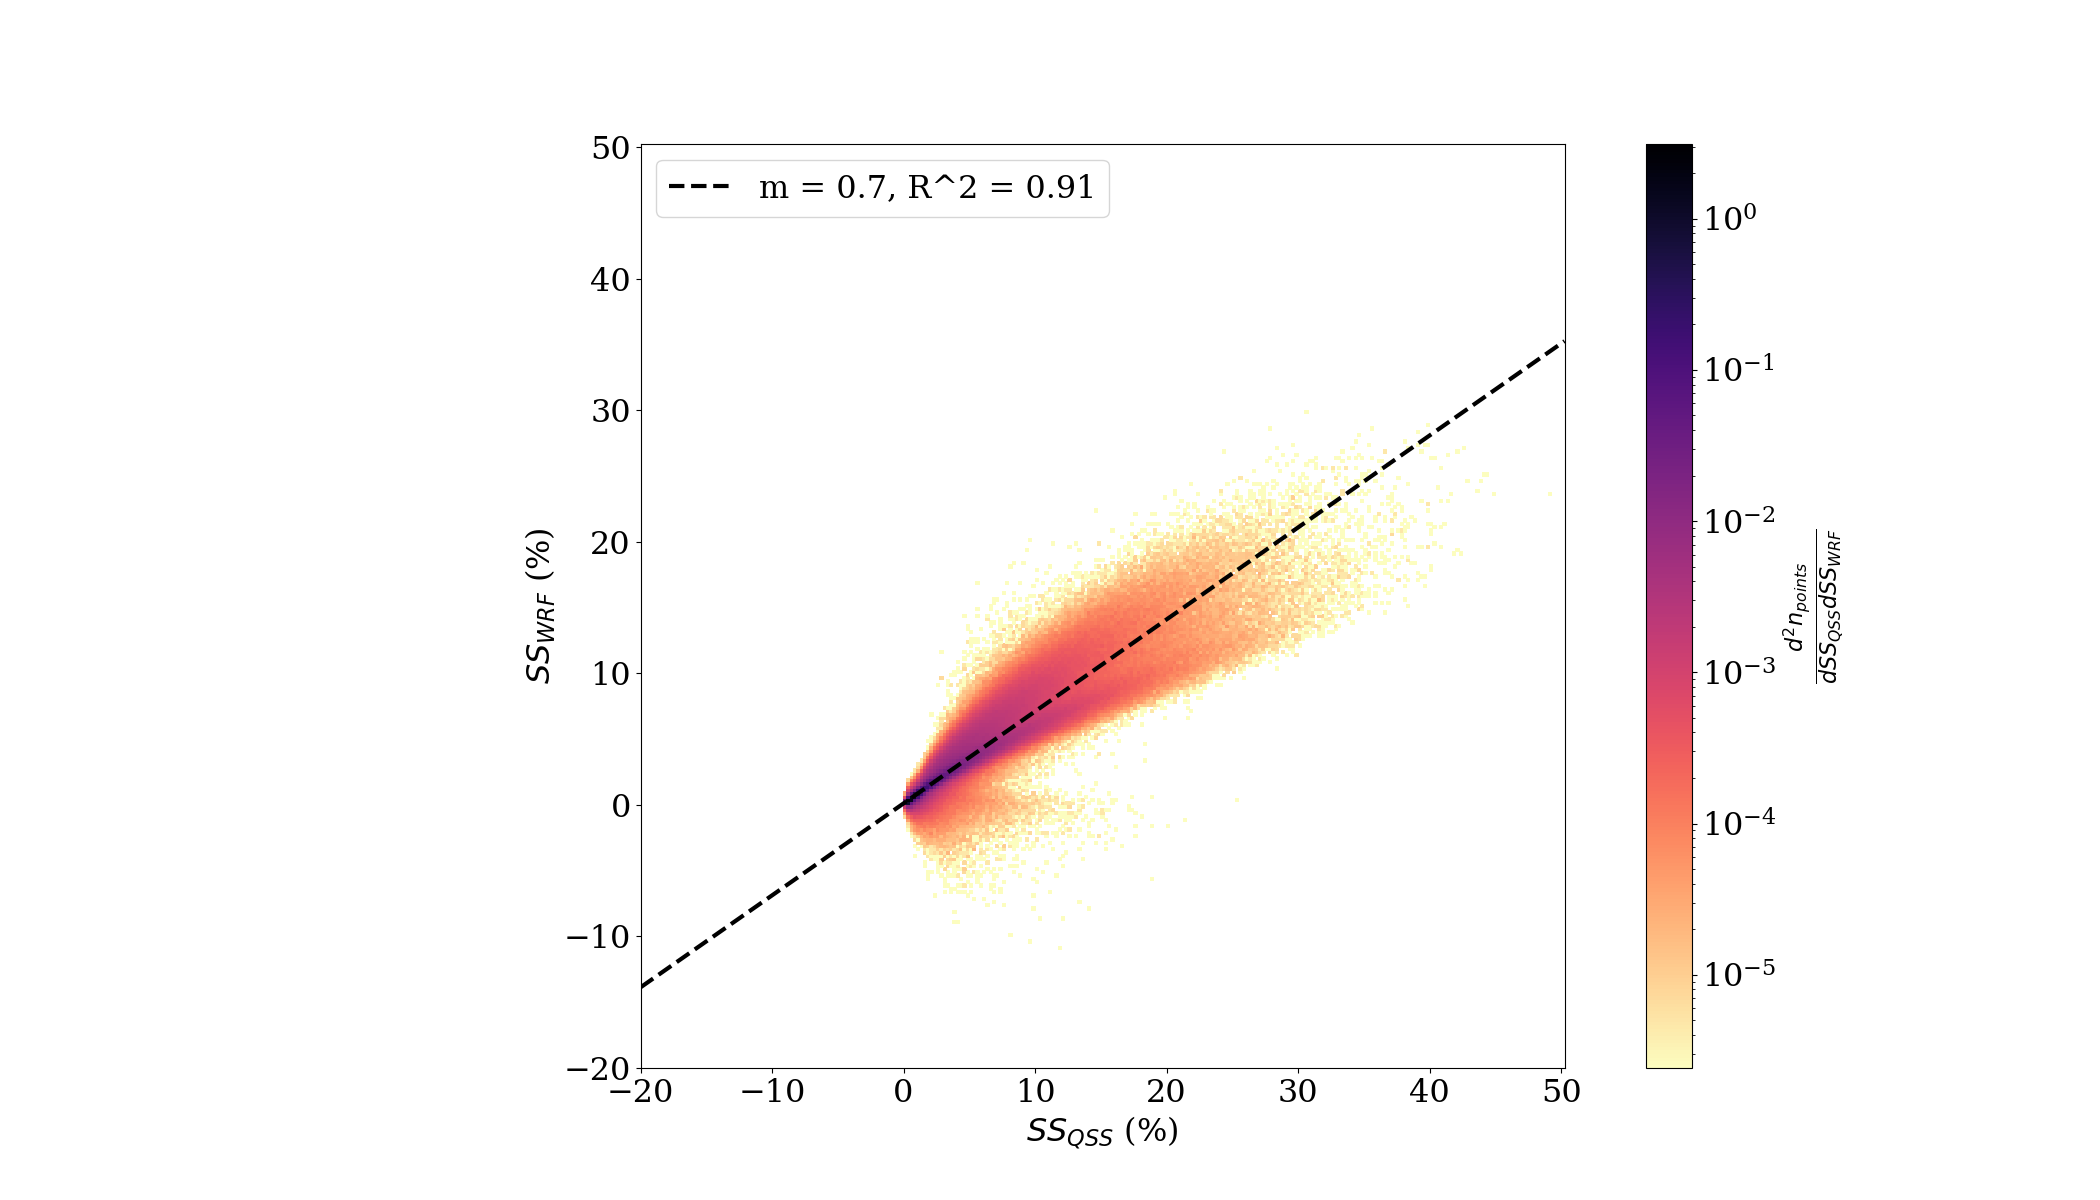
\includegraphics[width=\textwidth]{revmywrf/v11_FINAL_heatmap_ss_qss_vs_ss_wrf_Unpolluted_figure.png}
		\caption{Unpolluted case.}
		\label{wrfvsqssunpollv11}
	\end{subfigure}
	\begin{subfigure}{0.7\textwidth}
		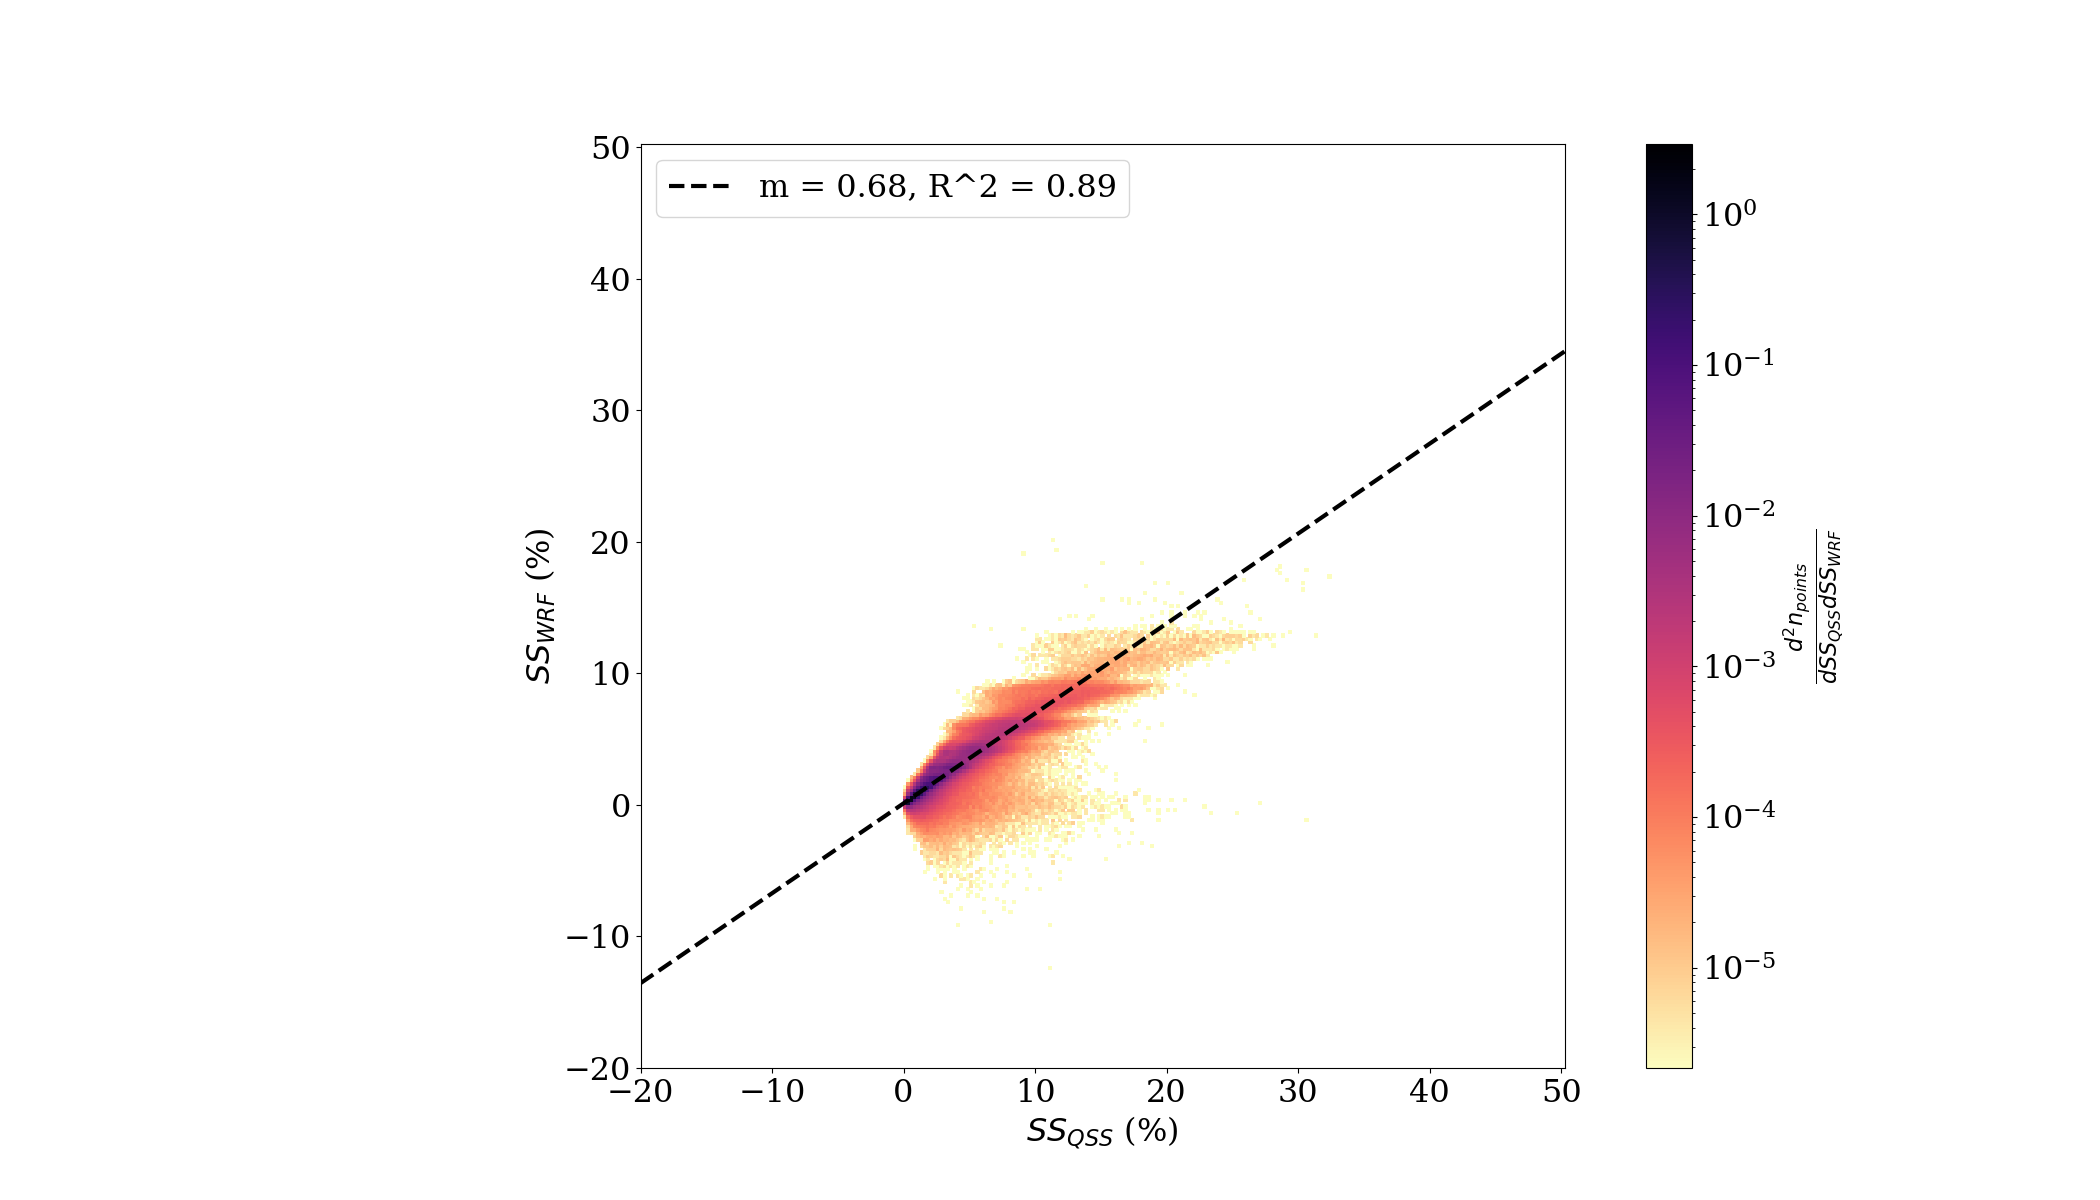
\includegraphics[width=\textwidth]{revmywrf/v11_FINAL_heatmap_ss_qss_vs_ss_wrf_Polluted_figure.png}
		\caption{Polluted case.}
		\label{wrfvsqsspollv11}
	\end{subfigure}
	\caption{Same as Figure \ref{wrfvsqss}, using simplified form of Equation \ref{fullss}. Correlation is not appreciably affected but the value of least-squares linear regression slopes is lower for both simulation cases.}
	\label{wrfvsqssv11}
\end{figure}

\begin{figure}[ht]
	\centering
	\begin{subfigure}{0.7\textwidth}
		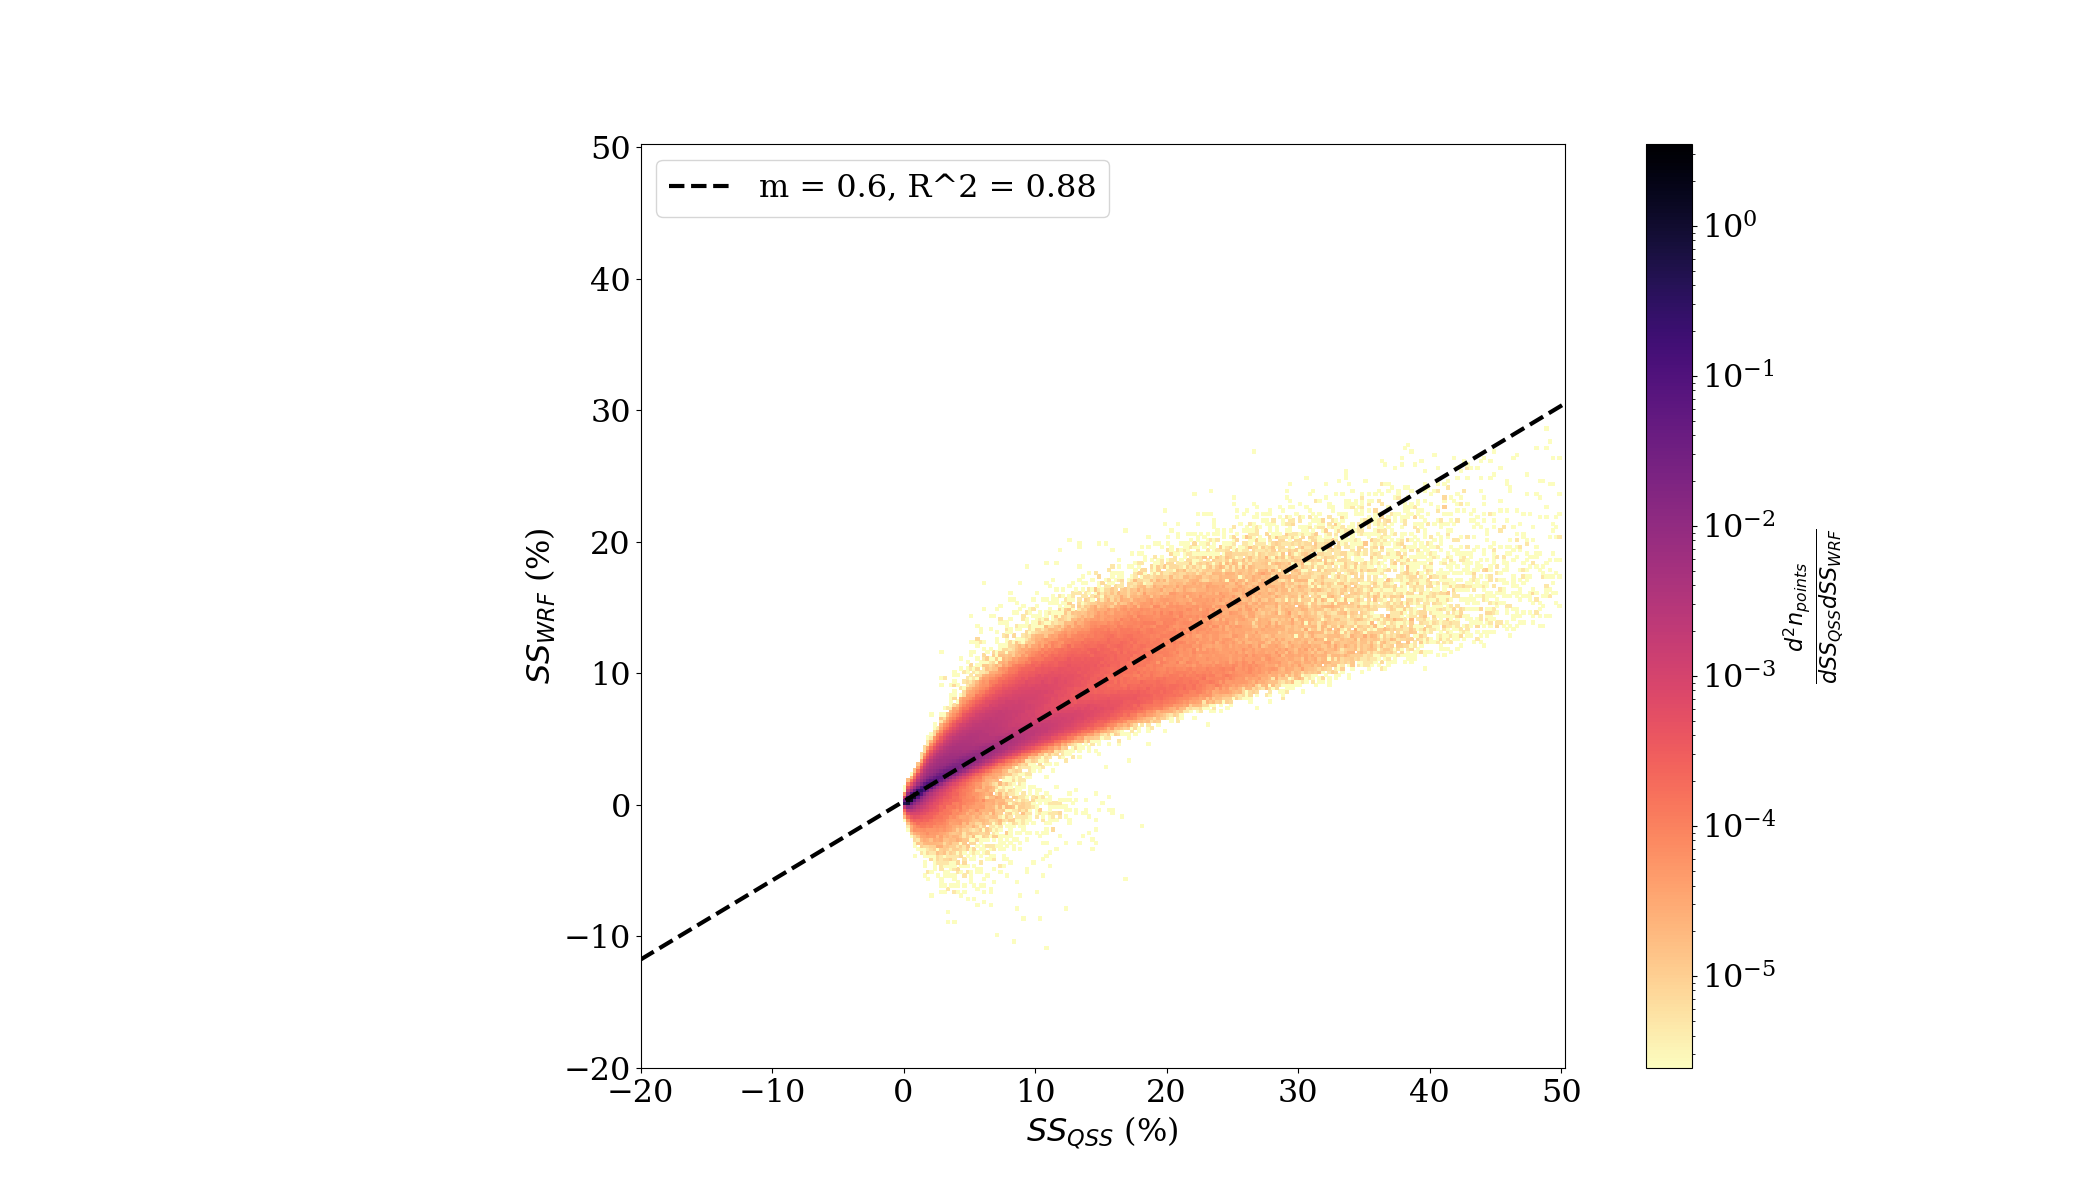
\includegraphics[width=\textwidth]{revmywrf/v12_FINAL_heatmap_ss_qss_vs_ss_wrf_Unpolluted_figure.png}
		\caption{Unpolluted case.}
		\label{wrfvsqssunpollv12}
	\end{subfigure}
	\begin{subfigure}{0.7\textwidth}
		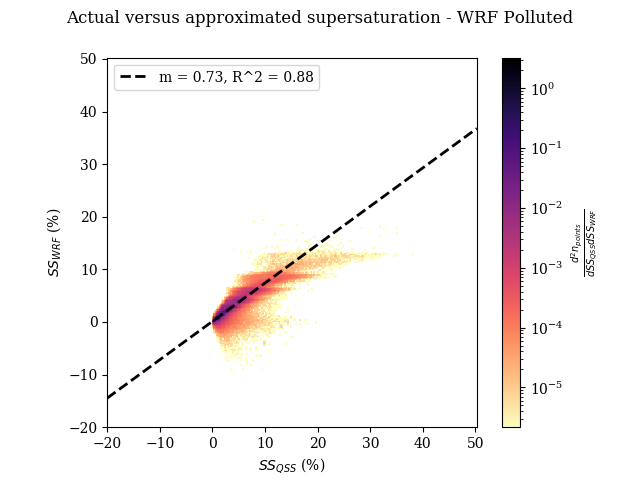
\includegraphics[width=\textwidth]{revmywrf/v12_FINAL_heatmap_ss_qss_vs_ss_wrf_Polluted_figure.png}
		\caption{Polluted case.}
		\label{wrfvsqsspollv12}
	\end{subfigure}
	\caption{Same as Figure \ref{wrfvsqss}, without ventilation corrections. Correlation is not appreciably affected but the value of least-squares linear regression slopes is lower for both simulation cases.}
	\label{wrfvsqssv12}
\end{figure}

\begin{figure}[ht]
	\centering
	\begin{subfigure}{0.7\textwidth}
		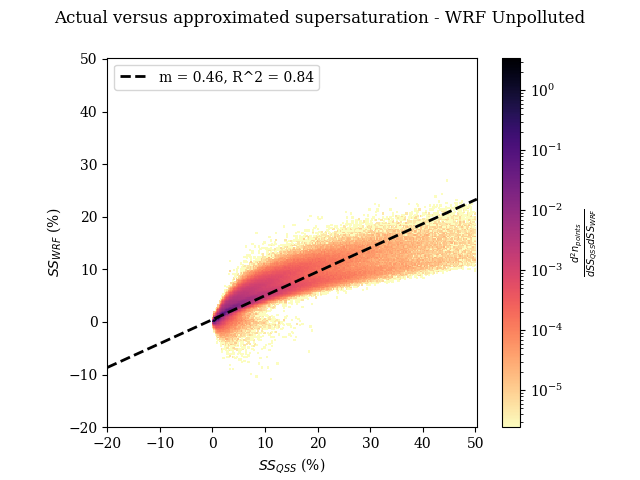
\includegraphics[width=\textwidth]{revmywrf/v13_FINAL_heatmap_ss_qss_vs_ss_wrf_Unpolluted_figure.png}
		\caption{Unpolluted case.}
		\label{wrfvsqssunpollv13}
	\end{subfigure}
	\begin{subfigure}{0.7\textwidth}
		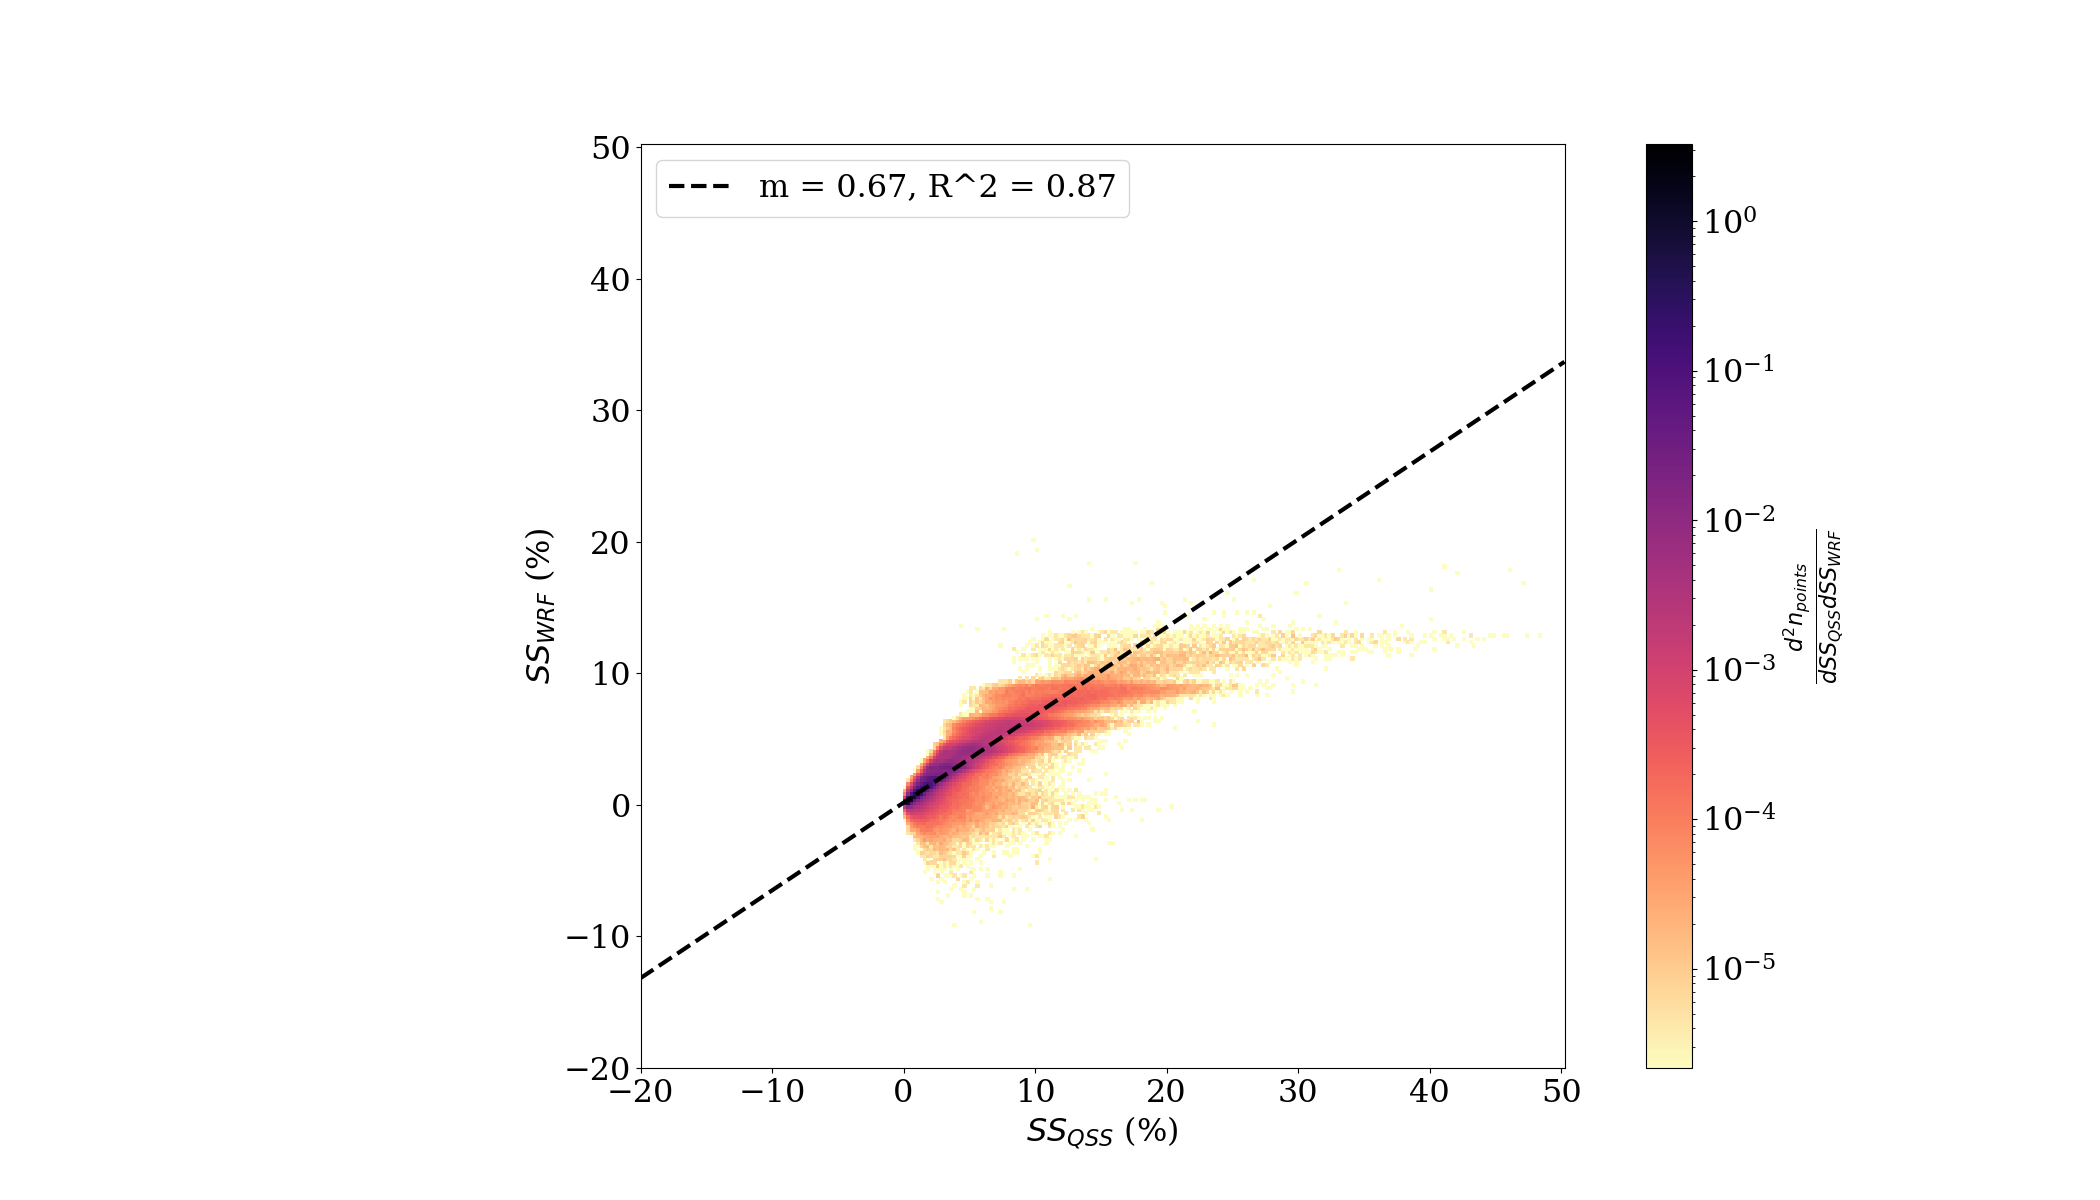
\includegraphics[width=\textwidth]{revmywrf/v13_FINAL_heatmap_ss_qss_vs_ss_wrf_Polluted_figure.png}
		\caption{Polluted case.}
		\label{wrfvsqsspollv13}
	\end{subfigure}
	\caption{Same as Figure \ref{wrfvsqss}, without contributions from rain drops. Correlation is slightly lower and the value of least-squared linear regression slopes is lower for both simulaiton cases.}
	\label{wrfvsqssv13}
\end{figure}

\begin{figure}[ht]
	\centering
	\begin{subfigure}{0.7\textwidth}
		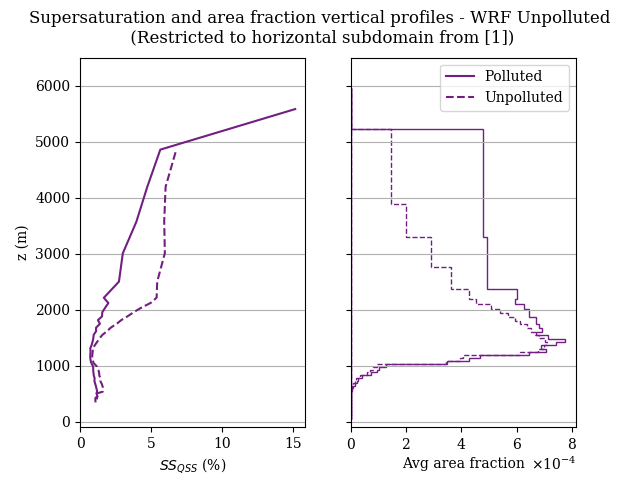
\includegraphics[width=\textwidth]{revmywrf/v3_FINAL_subdom_bipanel_ss_qss_vs_z_allpts_figure.png}
		\caption{}
		\label{wrfsubdombipanelallpts}
	\end{subfigure}
	\begin{subfigure}{0.7\textwidth}
		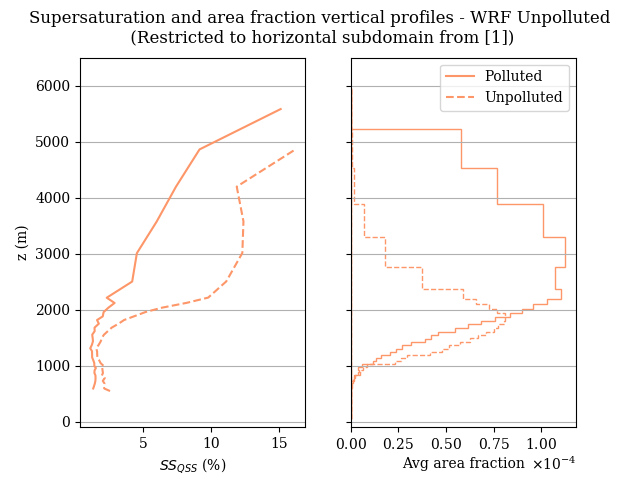
\includegraphics[width=\textwidth]{revmywrf/v3_FINAL_subdom_bipanel_ss_qss_vs_z_up10perc_figure.png}
		\caption{}
		\label{wrfsubdombipanelup50perc}
	\end{subfigure}
	\caption{Analagous to Figure \ref{wrfbipanel}, restricted to the horizontal subdomain indicated by the red box in Figure S8 of Fan et al (bottom left panel). Qualitatively the results are quite similar, suggesting that the restriction to this subdomain is not crucial to the results described in Fan's paper. TODO: Figure out why the form of the area fraction curve for the polluted simulation looks the way it does (not entirely clear just by looking at Figure \ref{subdomlwcprof}).}
	\label{wrfsubdombipanel}
\end{figure}

\begin{figure}[ht]
	\centering
	\begin{subfigure}{1\textwidth}
		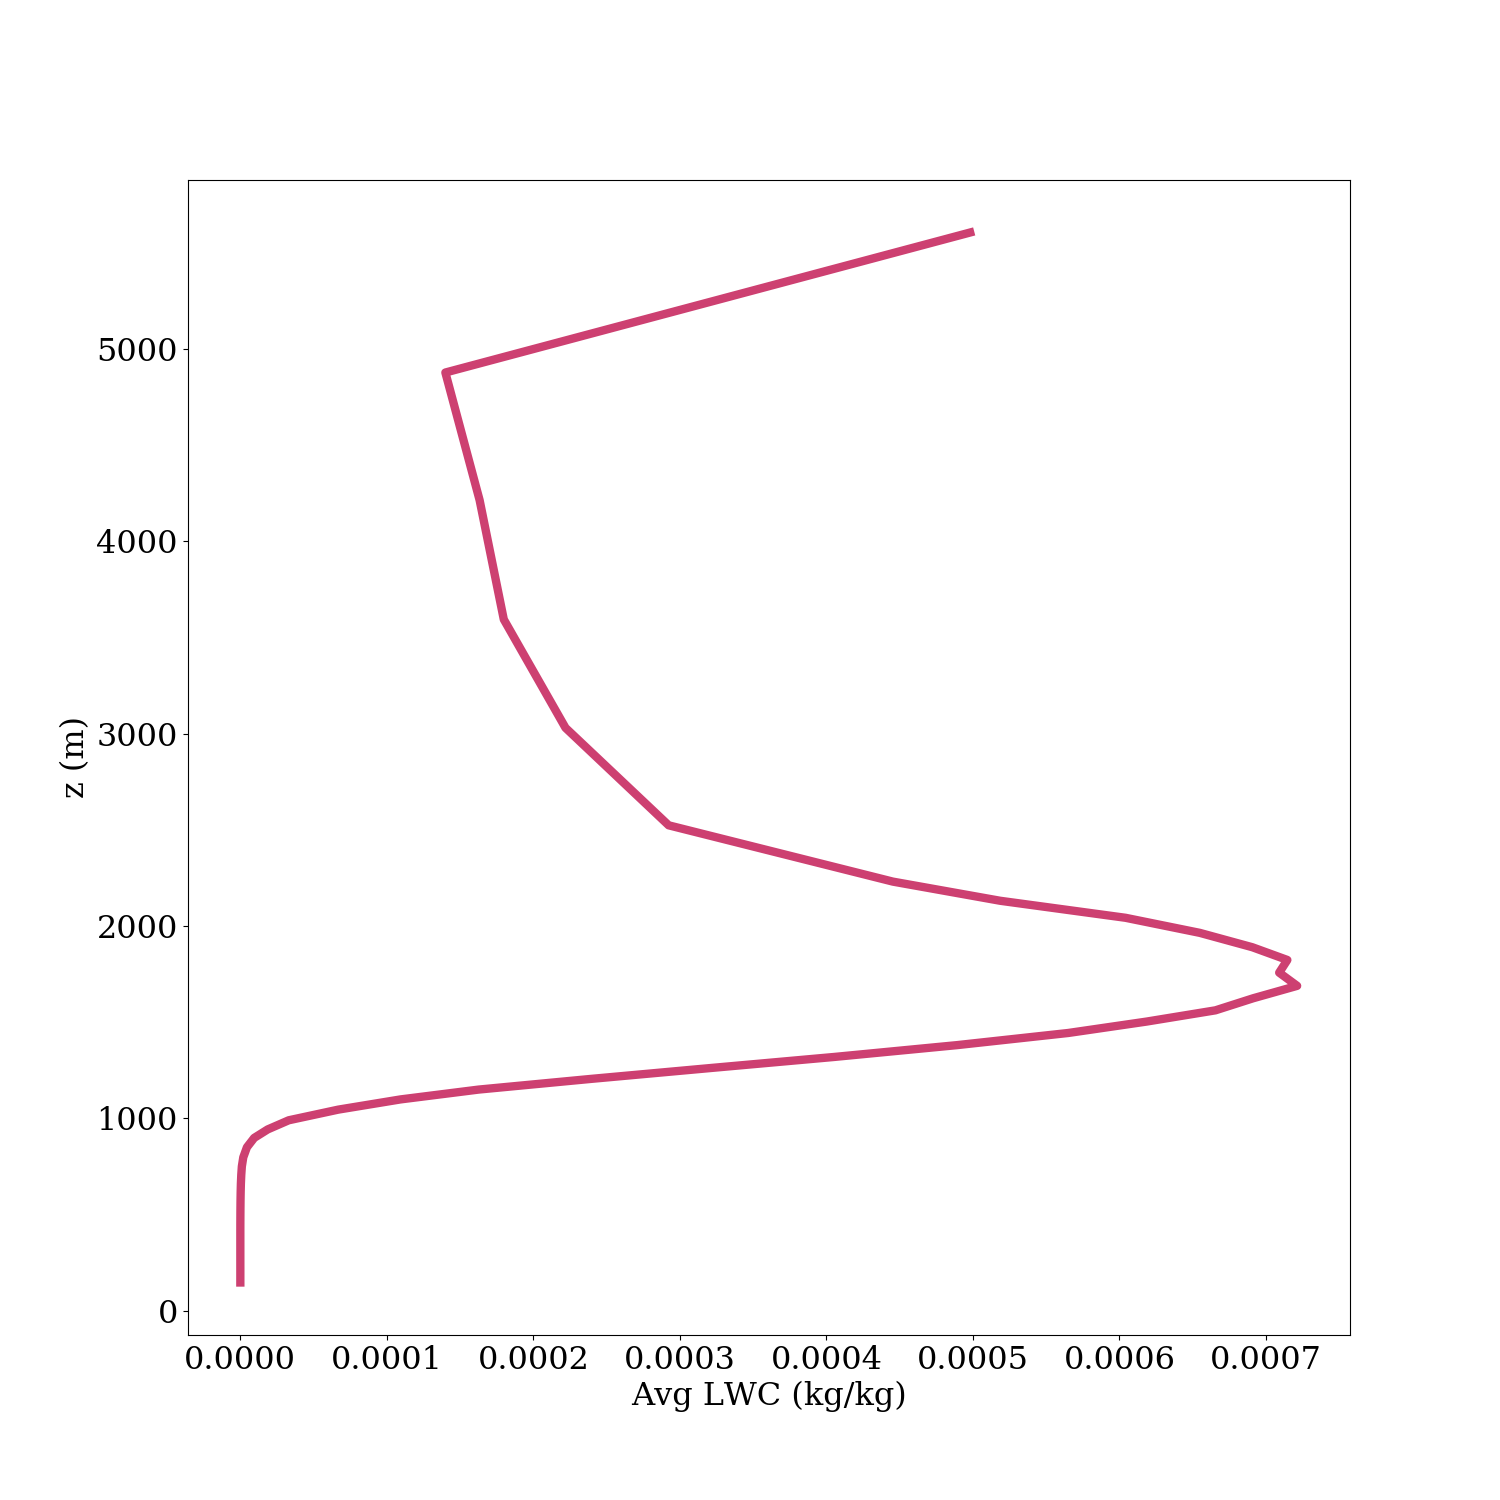
\includegraphics[width=\textwidth]{revmywrf/v1_lwc_vs_z_Unpolluted_figure.png}
		\caption{Unpolluted case.}
		\label{lwcprofunpoll}
	\end{subfigure}
	\begin{subfigure}{1\textwidth}
		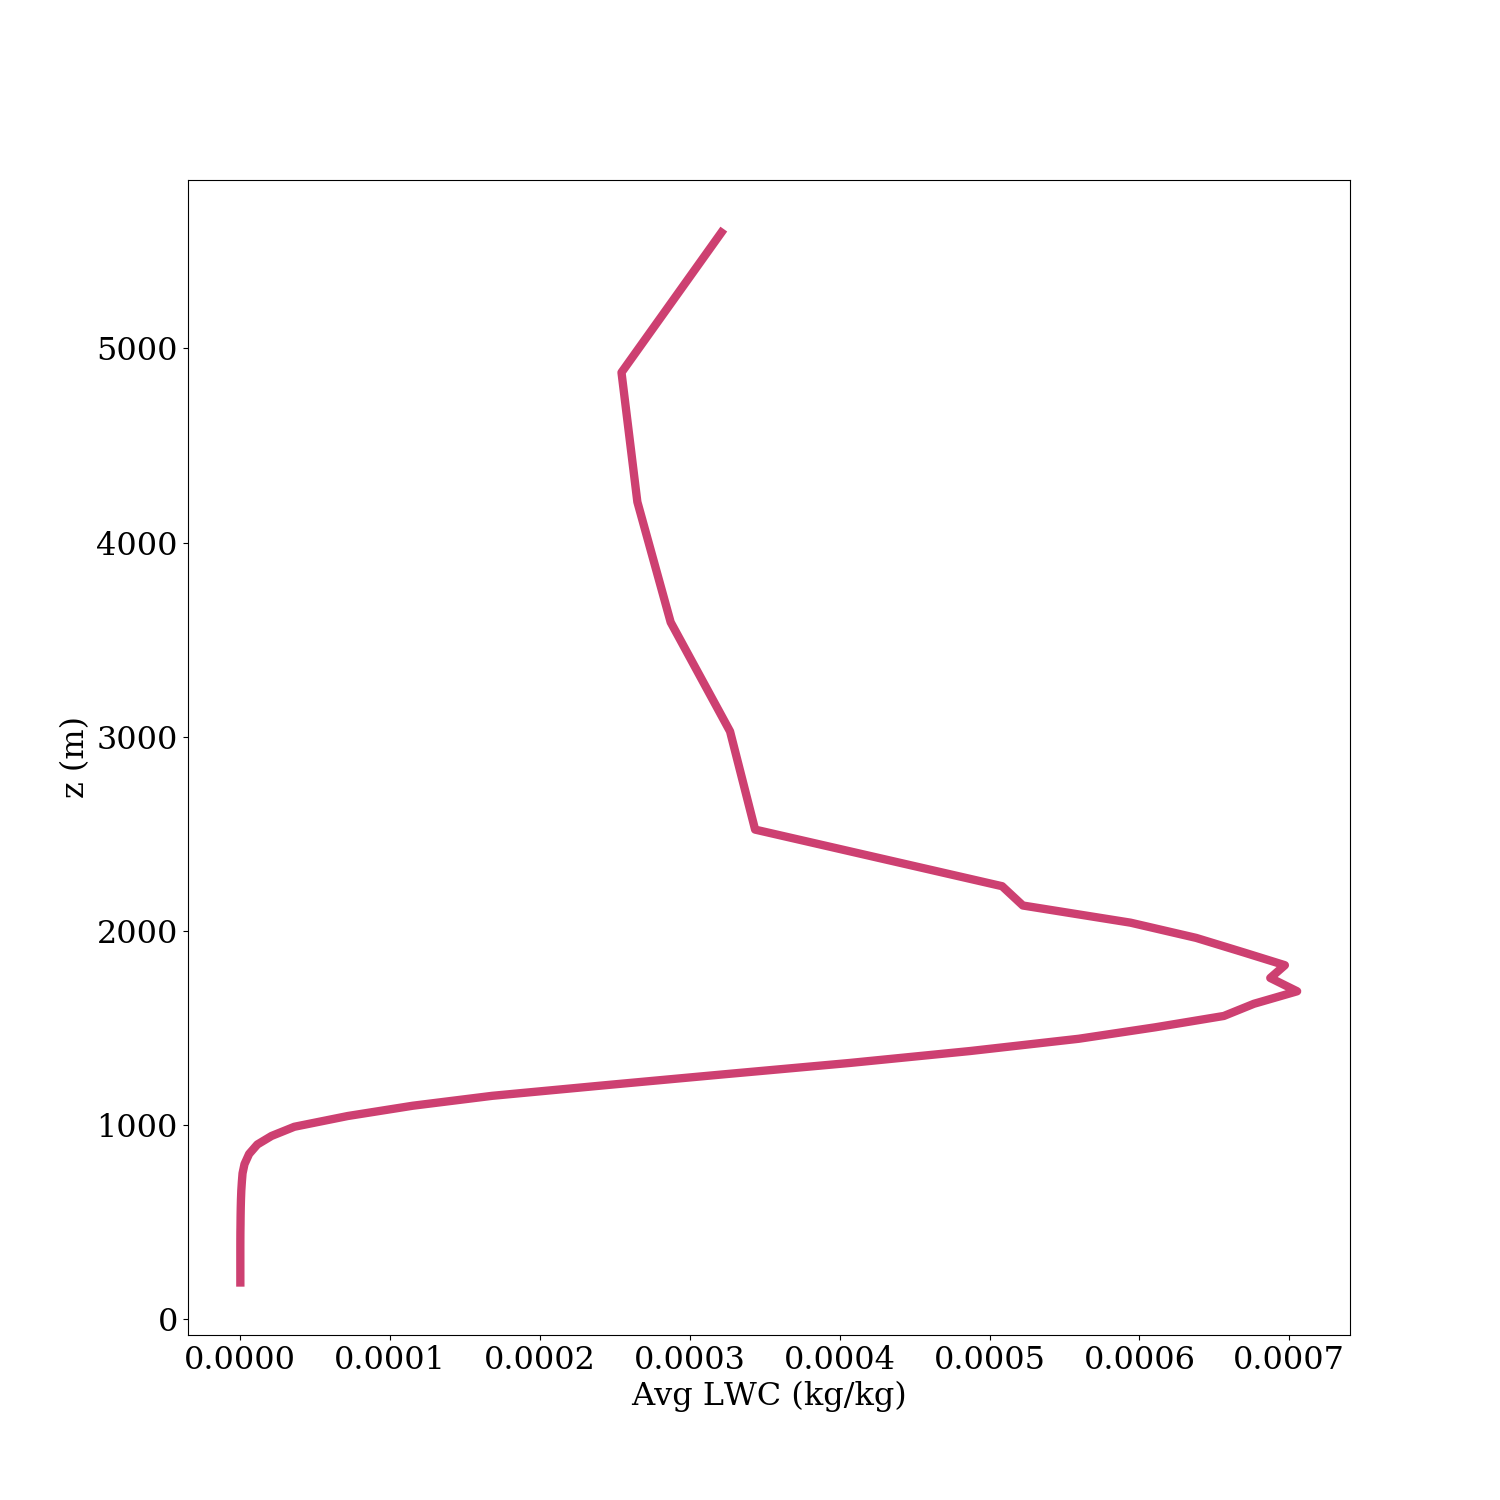
\includegraphics[width=\textwidth]{revmywrf/v1_lwc_vs_z_Polluted_figure.png}
		\caption{Polluted case.}
		\label{lwcprofpoll}
	\end{subfigure}
	\caption{Vertical $LWC$ profiles for the filtered WRF datasets. In both simulation cases, $LWC$ has a prominent peak between 2 and 3 km altitude.}
	\label{lwcprof}
\end{figure}

\begin{figure}[ht]
	\centering
	\begin{subfigure}{1\textwidth}
		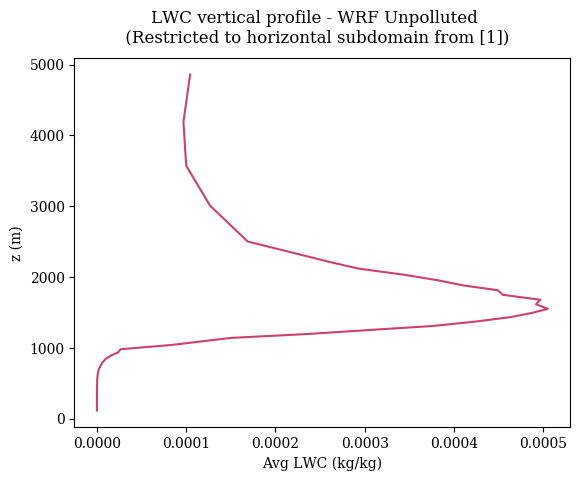
\includegraphics[width=\textwidth]{revmywrf/v1_subdom_lwc_vs_z_Unpolluted_figure.png}
		\caption{Unpolluted case.}
		\label{subdomlwcprofunpoll}
	\end{subfigure}
	\begin{subfigure}{1\textwidth}
		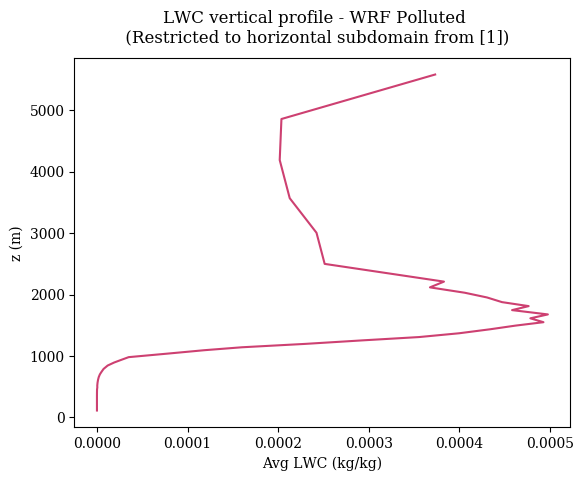
\includegraphics[width=\textwidth]{revmywrf/v1_subdom_lwc_vs_z_Polluted_figure.png}
		\caption{Polluted case.}
		\label{subdomlwcprofpoll}
	\end{subfigure}
	\caption{Analagous to Figure \ref{lwcprof}, restricted to the horizontal subdomain indicated by the red box in Figure S8 of Fan et al (bottom left panel).}
	\label{subdomlwcprof}
\end{figure}
\end{document}
